\chapter{MIGRAÇÃO}
\label{cap3}

A finalidade da migração é mover os eventos de reflexão registrados para a posição real na seção sísmica, de modo que a análise visual tenha uma correspondência direta com a estrutura do subsolo geológico.  
Esta operação pode ser realizada no domínio do tempo (domínio sísmico), ou do espaço denominada de profundidade (domínio geológico).
Devido a esta proposta fundamental, migração é também denominada de imageamento. 

A migração pós-empilhamento no tempo é um processo de imageamento de seções sísmicas empilhadas, e  objetivo é de focalizar a energia das difrações e reposicionando os refletores para a posição correta, o que resulta em aumentar a continuidade e a resolução lateral dos refletores. 

A migração no tempo leva em consideração o modelo ``refletor em explosão'', o que admite variações laterais suaves em subsuperfície.  

A migração das seções afastamento-nulo foi realizada com o método denominado de Migração Kirchhoff, onde  utilizamos o programa $sumigtk$ (ver anexo) do pacote CWP/SU \citep{STOCKWELL(2017)}.

\section{MIGRAÇÃO KIRCHHOFF NO TEMPO}

A migração Kirchhoff parte da solução da equação de onda na forma escalar dada por
\begin{equation}
\nabla^2 P(\mathbf{r},t)-\frac{1}{v^2}\frac{\partial^2 P(\mathbf{r},t)}{\partial t^2}=-4\pi q(\mathbf{r},t),
\label{eq:mig_kirchhoff_1}
\end{equation}
onde $P(\mathbf{r},t)$ é o campo de onda (amplitude), $v$ a velocidade constante do meio, $-4\pi q(\mathbf{r},t)$ representa a fonte, e $\mathbf{r}=\mathbf{r}(x, y, z)$ representa o ponto de observação.

A solução completa para a equação (\ref{eq:mig_kirchhoff_1}), para um volume sísmico $V_0$ delimitado por uma superfície $S_0$, é expressa pelo teorema de Green \citep{Schneider(1978)}, o que é dada por
\begin{equation}
P(\mathbf{r},t)=\frac{1}{4\pi}\int_{t_{0}}dt_0\int_{s_{0}} dS_0 \left[G\frac{\partial}{\partial n}P(\mathbf{r_0},t_0)-P(\mathbf{r_0},t_0)\frac{\partial}{\partial n}G\right],
\label{eq:mig_kirchhoff_2}
\end{equation}

onde $\mathbf{n}= n\hat{\mathbf{n}}$ é o vetor normal à superfície $S_0$, que inclui a superfície de aquisição $A_0$ e a superfície de forma semi-esférica $A'$ que é extrapolada para o infinito de forma que sua contribuição seja desprezível (ver Figura \ref{fig:migracao_kir1}).

Desta forma, os valores na fronteira se reduzem a uma integral na superfície de aquisição, e à função auxiliar de Green, $G(\mathbf{r},t|\mathbf{r_0},t_0)$, que consiste da resposta do meio a uma fonte pontual em $\mathbf{r_0}$. 
Neste caso a obtenção da função de Green utiliza o método das imagens, que para uma superfície plana localiza a imagem no ponto $\mathbf{r'_0}$, e para um semi-espaço ela é dada por 

\begin{equation}
G(\mathbf{r},t|\mathbf{r_0},t_0)=\frac{\delta(t-t_{0}-\frac{R}{v})}{R}-\frac{\delta(t-t_{0}-\frac{R'}{v})}{R'},
\label{eq:mig_kirchhoff_3}
\end{equation}
onde

\begin{equation}
R=[(x-x_0)^2+(y-y_0)^2+(z-z_0)^2]^{\frac{1}{2}},
\label{eq:mig_kirchhoff_4}
\end{equation}
\begin{equation}
R'=[(x-x_0)^2+(y-y_0)^2+(z+z_0)^2]^{\frac{1}{2}}.
\label{eq:mig_kirchhoff_5}
\end{equation}


\begin{figure}[H]
\centering
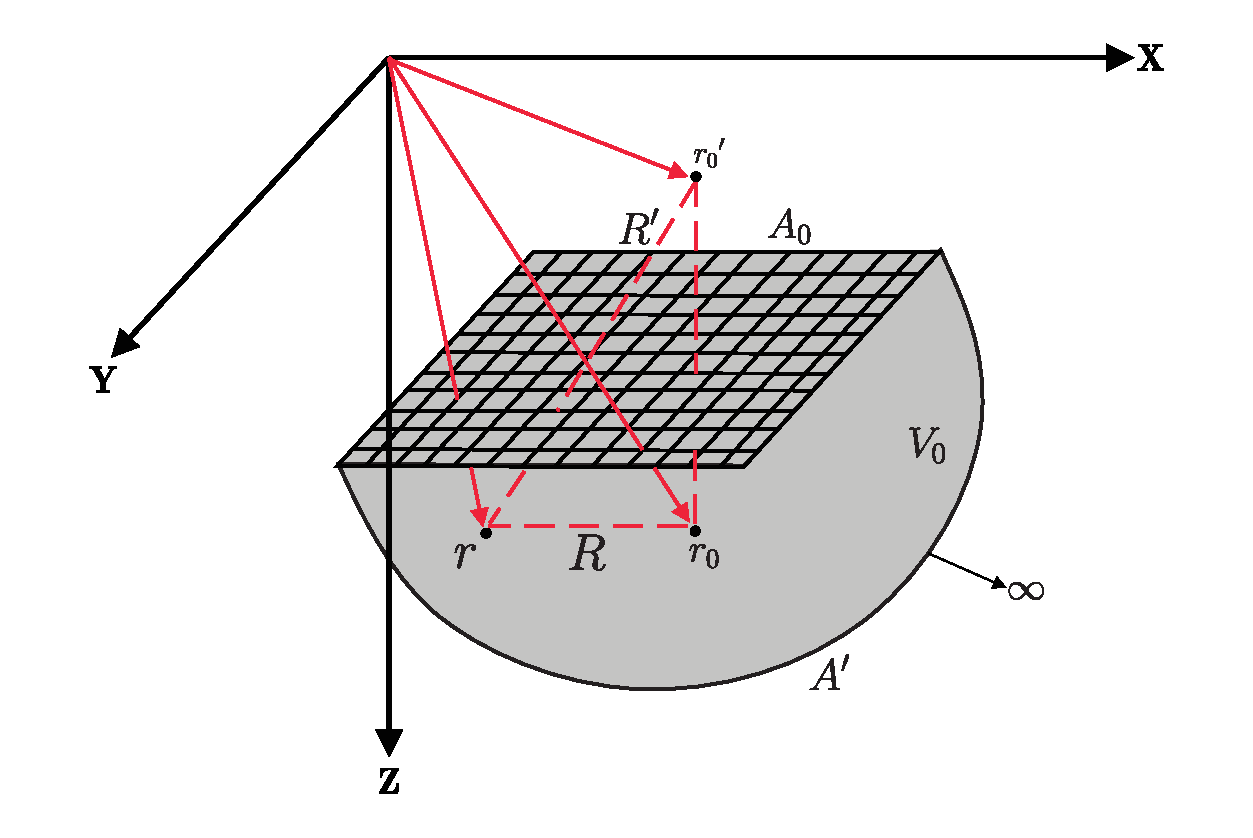
\includegraphics[totalheight=9.0cm]{figuras/cap3/migracao_kir1.pdf}
\caption{Meio escalar (3D) com volume $V_0$ delimitado pela fronteira $S_0 = A_0 + A'$, com um ponto fonte incluso em $\mathbf{r_0}$, sua imagem em $\mathbf{r'_0}$, e um ponto de observação em 
$\mathbf{r'}$. Fonte: Modificado de \citep{Schneider(1978)}.}
\label{fig:migracao_kir1}
\end{figure}

Na construção sísmica do problema, o campo $P(\mathbf{r_0},t)$ é medido na fronteira $S_0 = A_0 + A'$, onde a função de Green se anula ($G = 0$), e é uma forma de eliminar a componente $\frac{\partial P(\mathbf{r_0},t_0)}{\partial n}$ na integral, e se admite que $\mathbf{n}$ corresponde à vertical $\mathbf{z}$; ou seja, $n\rightarrow z_0$ (disto vem o conceito de migração em profundidade). 
Sendo assim, a equação (\ref{eq:mig_kirchhoff_2}) é simplificada à forma

\begin{equation}
P(\mathbf{r},t)=\frac{1}{2\pi}\int_{t_0}dt_0\int_{A_0}dA_0\left\{P(\mathbf{r_0},t_0)\frac{\partial}{\partial z_0}\left[\frac{\delta (t-t_0-\frac{R}{v})}{R} \right]\right\},
\label{eq:mig_kirchhoff_6}
\end{equation}
sendo denominada de integral de Kirchhoff para a migração em profundidade. 

Resolvendo a parte temporal da equação (\ref{eq:mig_kirchhoff_6}) que contém a função Delta de Dirac, e depois substituindo convenientemente $\frac{\partial}{\partial z_0}$ por $\frac{\partial}{\partial z}$,  resulta em
\begin{equation}
P(\mathbf{r},t)=-\frac{1}{\pi}\frac{\partial}{\partial z}\int_{A_0}dA_0\frac{P(\mathbf{r_0},t-\frac{R}{v})}{R}
\label{eq:mig_kirchhoff_7}
\end{equation}
Esta representação mostra que a equação (\ref{eq:mig_kirchhoff_1}) é solução da equação da onda em virtude da forma $\frac{f(t-\frac{R}{v})}{R}$ do integrando.

Uma forma de representar uma seção sísmica empilhada é através do experimento físico denominado \textit{refletor-em-explosão}. 
Neste modelo onde os receptores são localizados numa superfície de aquisição, e as fontes ao longo das interfaces refletoras onde são acionadas simultaneamente no instante de tempo $t=0$, de onde o campo produzido se propaga até a superfície de aquisição segundo o Princípio de Huygens (ver Figura \ref{fig:refletor-em-explosao}).
Neste modelo, as equações ao longo desta seção devem ter suas velocidades alteradas ou o tempo pelo fator $1/2$, e o resultado é a velocidade de migração (ver Figura \ref{fig:refletor-em-explosao2}).

\begin{figure}[H]
\centering
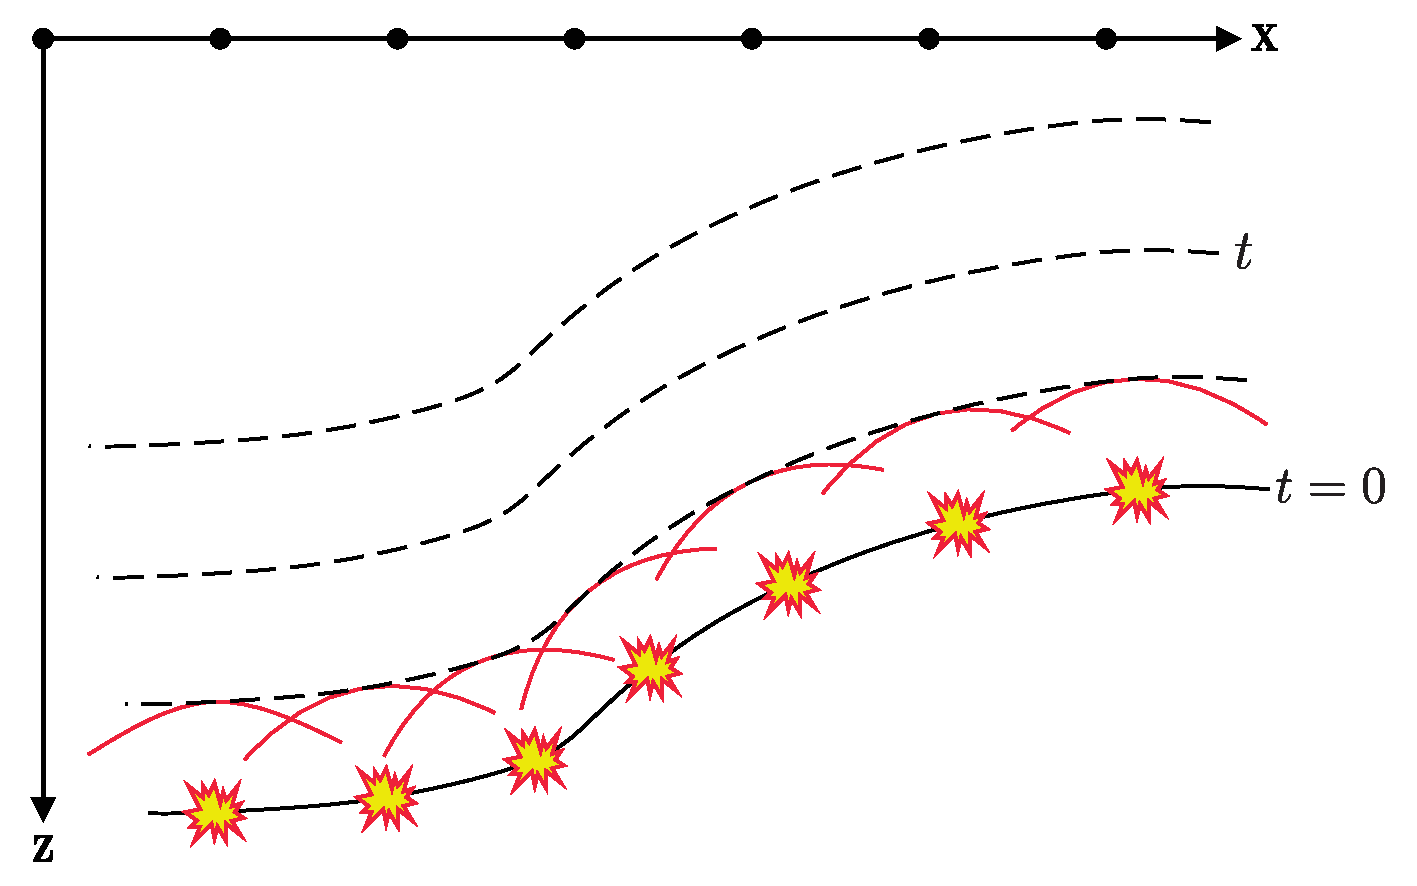
\includegraphics[totalheight=7.0cm]{figuras/cap3/refletor-em-explosao.pdf}
\caption{Representação do modelo refletor-em-explosão (em 2D para facilitar o desenho). 
As fontes estão localizadas nas interfaces refletoras são acionadas simultaneamente. 
O campo produzido se propaga de acordo com o Princípio de Huygens até a superfície de aquisição $z=0$. Fonte: Modificado de \citep{Schneider(1978)}}
\label{fig:refletor-em-explosao}
\end{figure}

\begin{figure}[H]
\centering
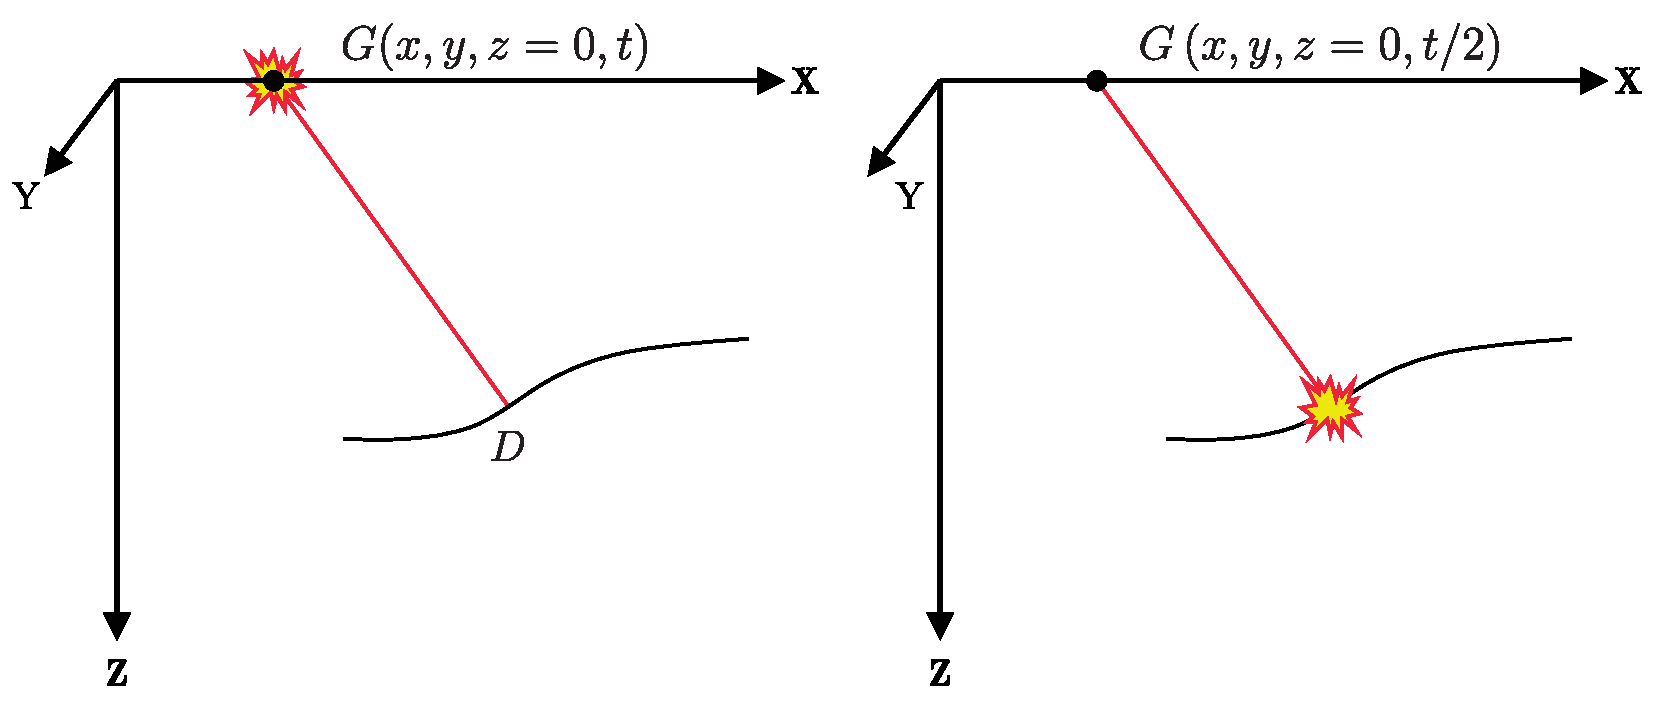
\includegraphics[totalheight=6.0cm]{figuras/cap3/refletor-em-explosao3.pdf}
\caption{Modelo afastamento-nulo (esquerda) e do \textit{refletor-em-explosão} (direita). 
Na esquerda o campo de onda parte da superfície no instante $t=0$, reflete em D e retorna a superfície onde é registrado no tempo de percurso duplo (desce-e-sobe), $t$. 
Na direita se tem outra forma de representar o afastamento-nulo equivalente, onde o campo de onda parte de um ponto da subsuperfície em $t=0$ e é registrado na superfície no tempo $t/2$. 
O conceito diz que a velocidade do campo de onda no modelo afastamento-nulo (esquerda) é a metade da velocidade do campo de onda no modelo do \textit{refletor-em-explosão} (direita). 
Fonte Modificado de \citep{Schneider(1978)}.}
\label{fig:refletor-em-explosao2}
\end{figure}

Dada uma seção empilhada pode-se continuar em profundidade o dado registrado $P(x,y,z=0,t)$, o que é representado pela equação
\begin{equation}
P(x,y,z,t)=-\frac{1}{2\pi}\frac{\partial}{\partial z}\int_{A_0}dA_0\frac{P(x,y,z=0,t+\frac{R}{v})}{R}. 
\label{eq:mig_kirchhoff_8}
\end{equation}

Usualmente se deseja modelar a magnitude para a fonte-em-explosão proporcional à refletividade da interface, e para isto se calcula a equação (\ref{eq:mig_kirchhoff_8}) para os pontos em subsuperfície no tempo $t=0$ de acionamento das fontes. 
Fixando $t=0$ e calculando a integral para toda área de interesse $(x,y,z)$, ou seja,

\begin{equation}
P(x,y,z,t=0)=-\frac{1}{2\pi}\frac{\partial}{\partial z}\int_{x_0}\int_{y_0}dx_0 dy_0\frac{P(x,y,z=0,\frac{R}{v})}{R}.
\label{eq:mig_kirchhoff_9}
\end{equation}


Este processo é denominado migração pós-empilhamento (seções afastamento-nulo, ou seções de incidência normal) baseado na integral de Kirchhoff, ou simplesmente migração Kirchhoff.
A equação (\ref{eq:mig_kirchhoff_9}) corresponde ao modelo da seção migrada (continuada) conhecida como \textit{condição de imagem} que mapea o campo no domínio $(x,y,z,t)$ para o domínio $(x,y,z)$, e que também pode ser mapeado para o domínio $(x,y,z,t=\frac{z}{v})$ correspondente à uma continuidade em profundidade (subsuperfície).
A figura \ref{fig:mapeamento_mig} exibe a relação entre o dado de entrada e o de saída no processo de mapeamento.

A entrada é um traço empilhado registrado no plano $z=0$, e a saída é um traço em uma posição ($x,y$) plotado em função de $z$ e do tempo $t=\frac{z}{v}$. 
Como os refletores se distribuem de cima para baixo através de sucessivas posições, imagea-se um ponto em cada uma destas etapas, se calculando a integral para cada um ponto para o tempo $t=0$. 
Exemplificando, o receptor $r_1$ em $z_1$ mapea um valor nulo para $t=0$ devido o receptor não estar no ponto de reflexão, da mesma forma o valor é anulado para o receptor $r_2$ em $z_2$. O valor numérico desta integral não será nulo quando o receptor estiver muito próximo ou em cima do refletor, como ocorre em $z_3$, quando isto ocorre um valor não-nulo é relacionado a este determinado ponto na subsuperfície, este mapeamento é a última etapa do processo da migração Kirchhoff, e assim produzirá uma imagem migrada (por continuação para baixo).

\begin{figure}[H]
\centering
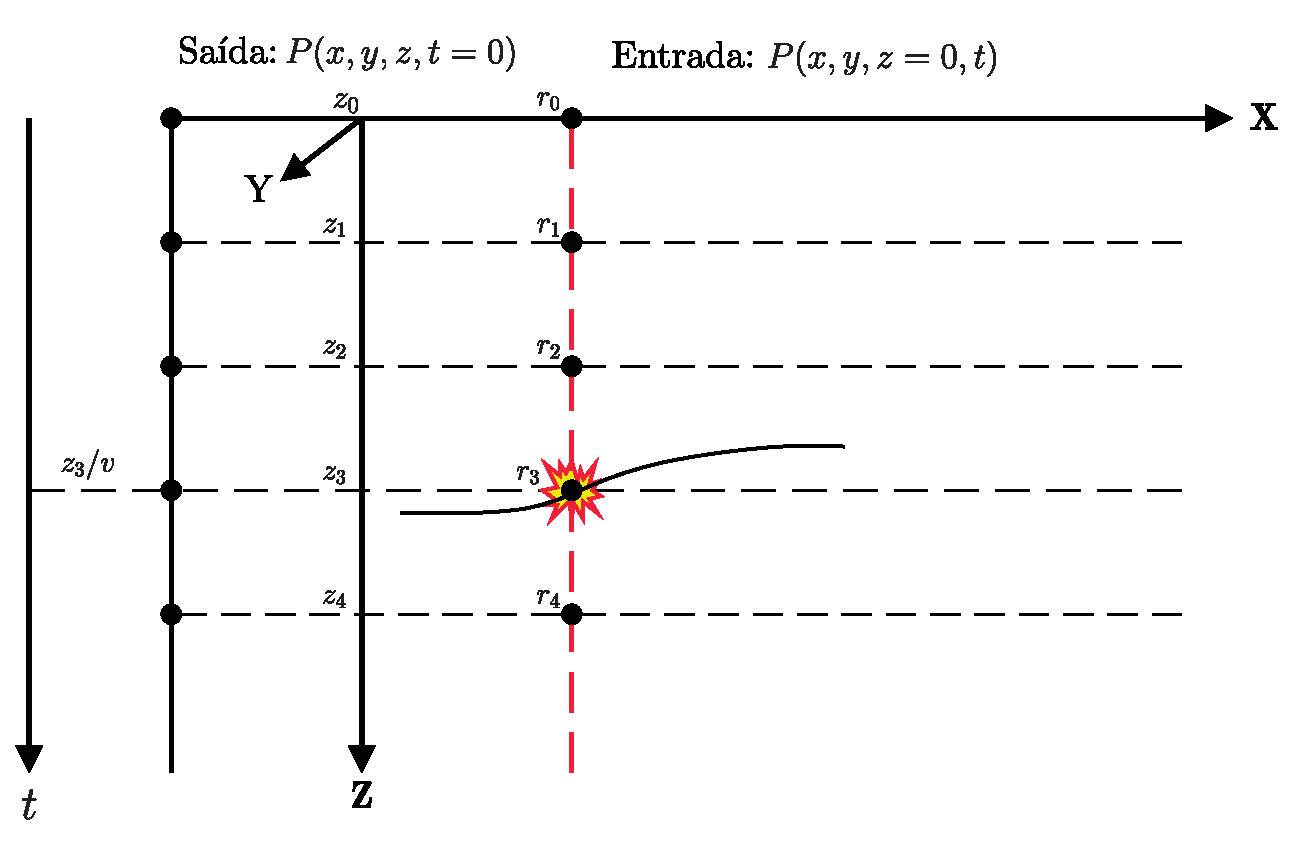
\includegraphics[totalheight=9.0cm]{figuras/cap3/mapeamento_mig.pdf}
\caption{A relação entre o dado de entrada $P(x,y,z=0,t)$ e o dado de saída $P(x,y,z,t=0)$. 
O mapeamento do campo de onda sísmico $(x,y,z,t)$ para $(x,y,z,t=\frac{z}{v})$. 
Observe que o modelo de velocidade admite apenas $v=v(z)$, mas na realidade $v=v(x,y,z)$.
Fonte: Modificado de \citep{Schneider(1978)}.}
\label{fig:mapeamento_mig}
\end{figure}

Sendo assim, segundo o modelo do \textit{refletor-em-explosão} e o processo de migração, a equação (\ref{eq:mig_kirchhoff_9}) é entendida como o processo que permite conhecer o valor do campo no tempo $t=0$ a partir de seus valores registrados pelos receptores no tempo $t$. 
Ou também, como um processo de continuação do campo de onda $P(\mathbf{r_0},t_0)$, conhecido na fronteira $A_0$, para $P(\mathbf{r},t=0)$ em um ponto na subsuperfície.

\begin{landscape}
\begin{figure}[H]
\centering
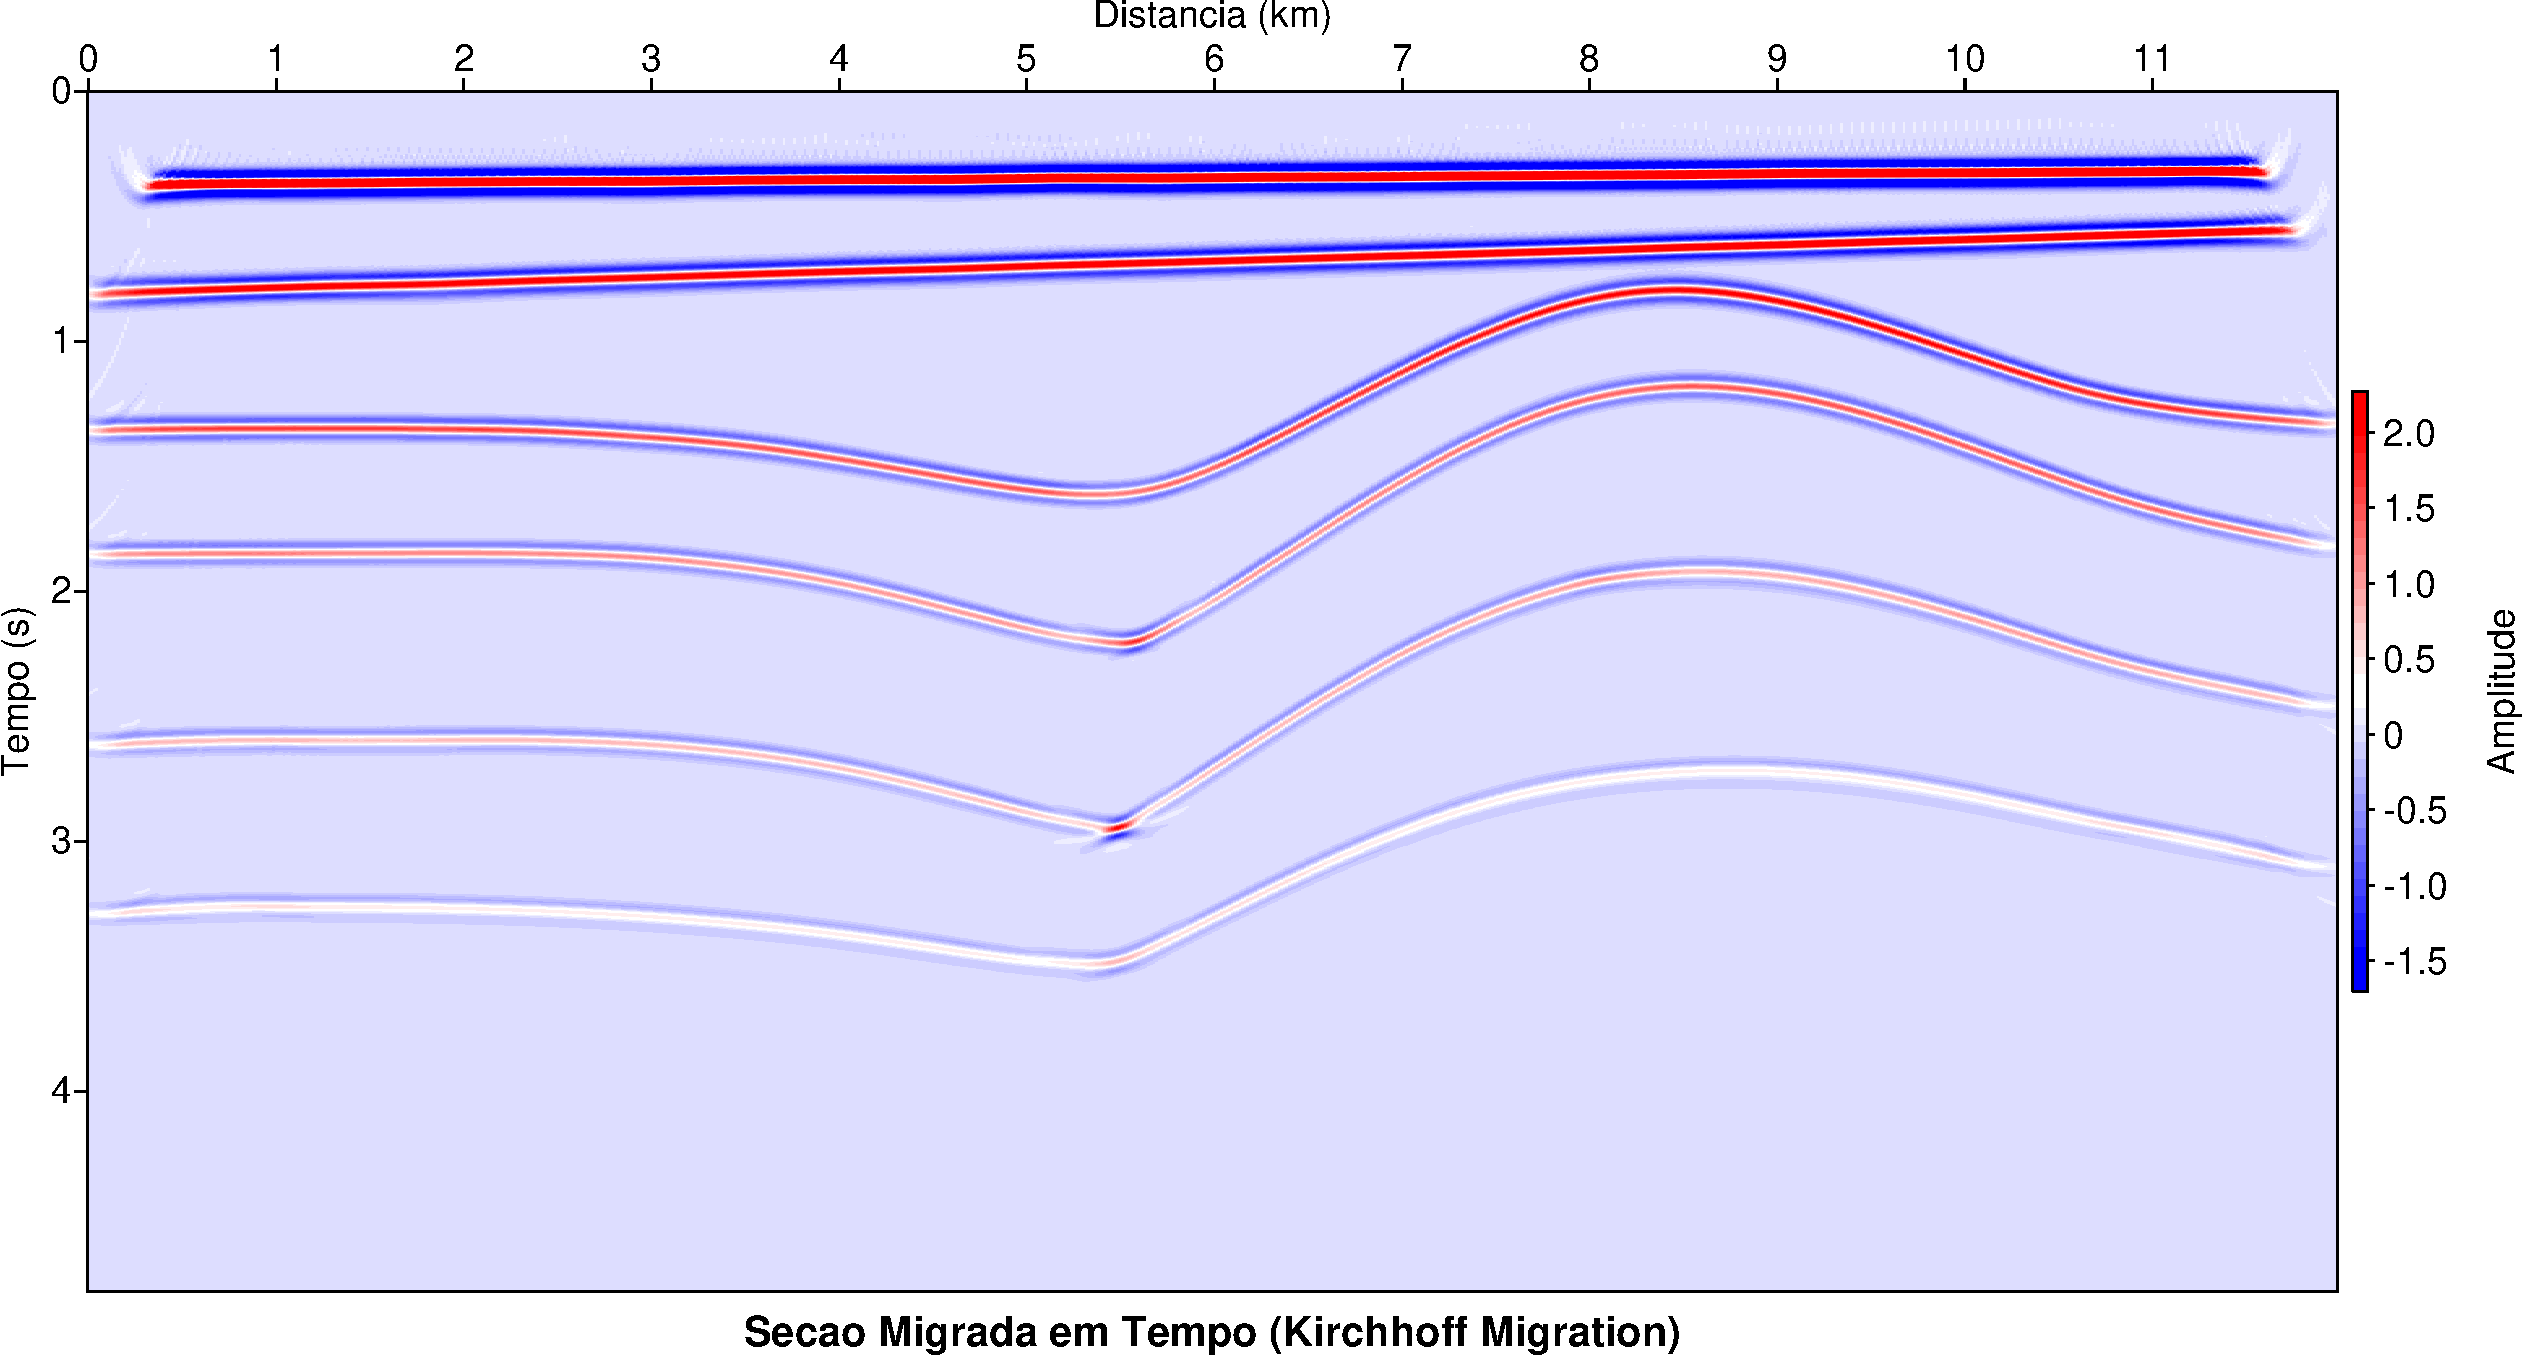
\includegraphics[totalheight=14cm]{figuras/cap3/seis_mig.pdf}
\caption{Seção migrada em tempo pelo método Kirchhoff utilizando o modelo de velocidade suavizado.}
\label{fig:seis_mig}
\end{figure}
\end{landscape}

\begin{landscape}
\begin{figure}[H]
\centering
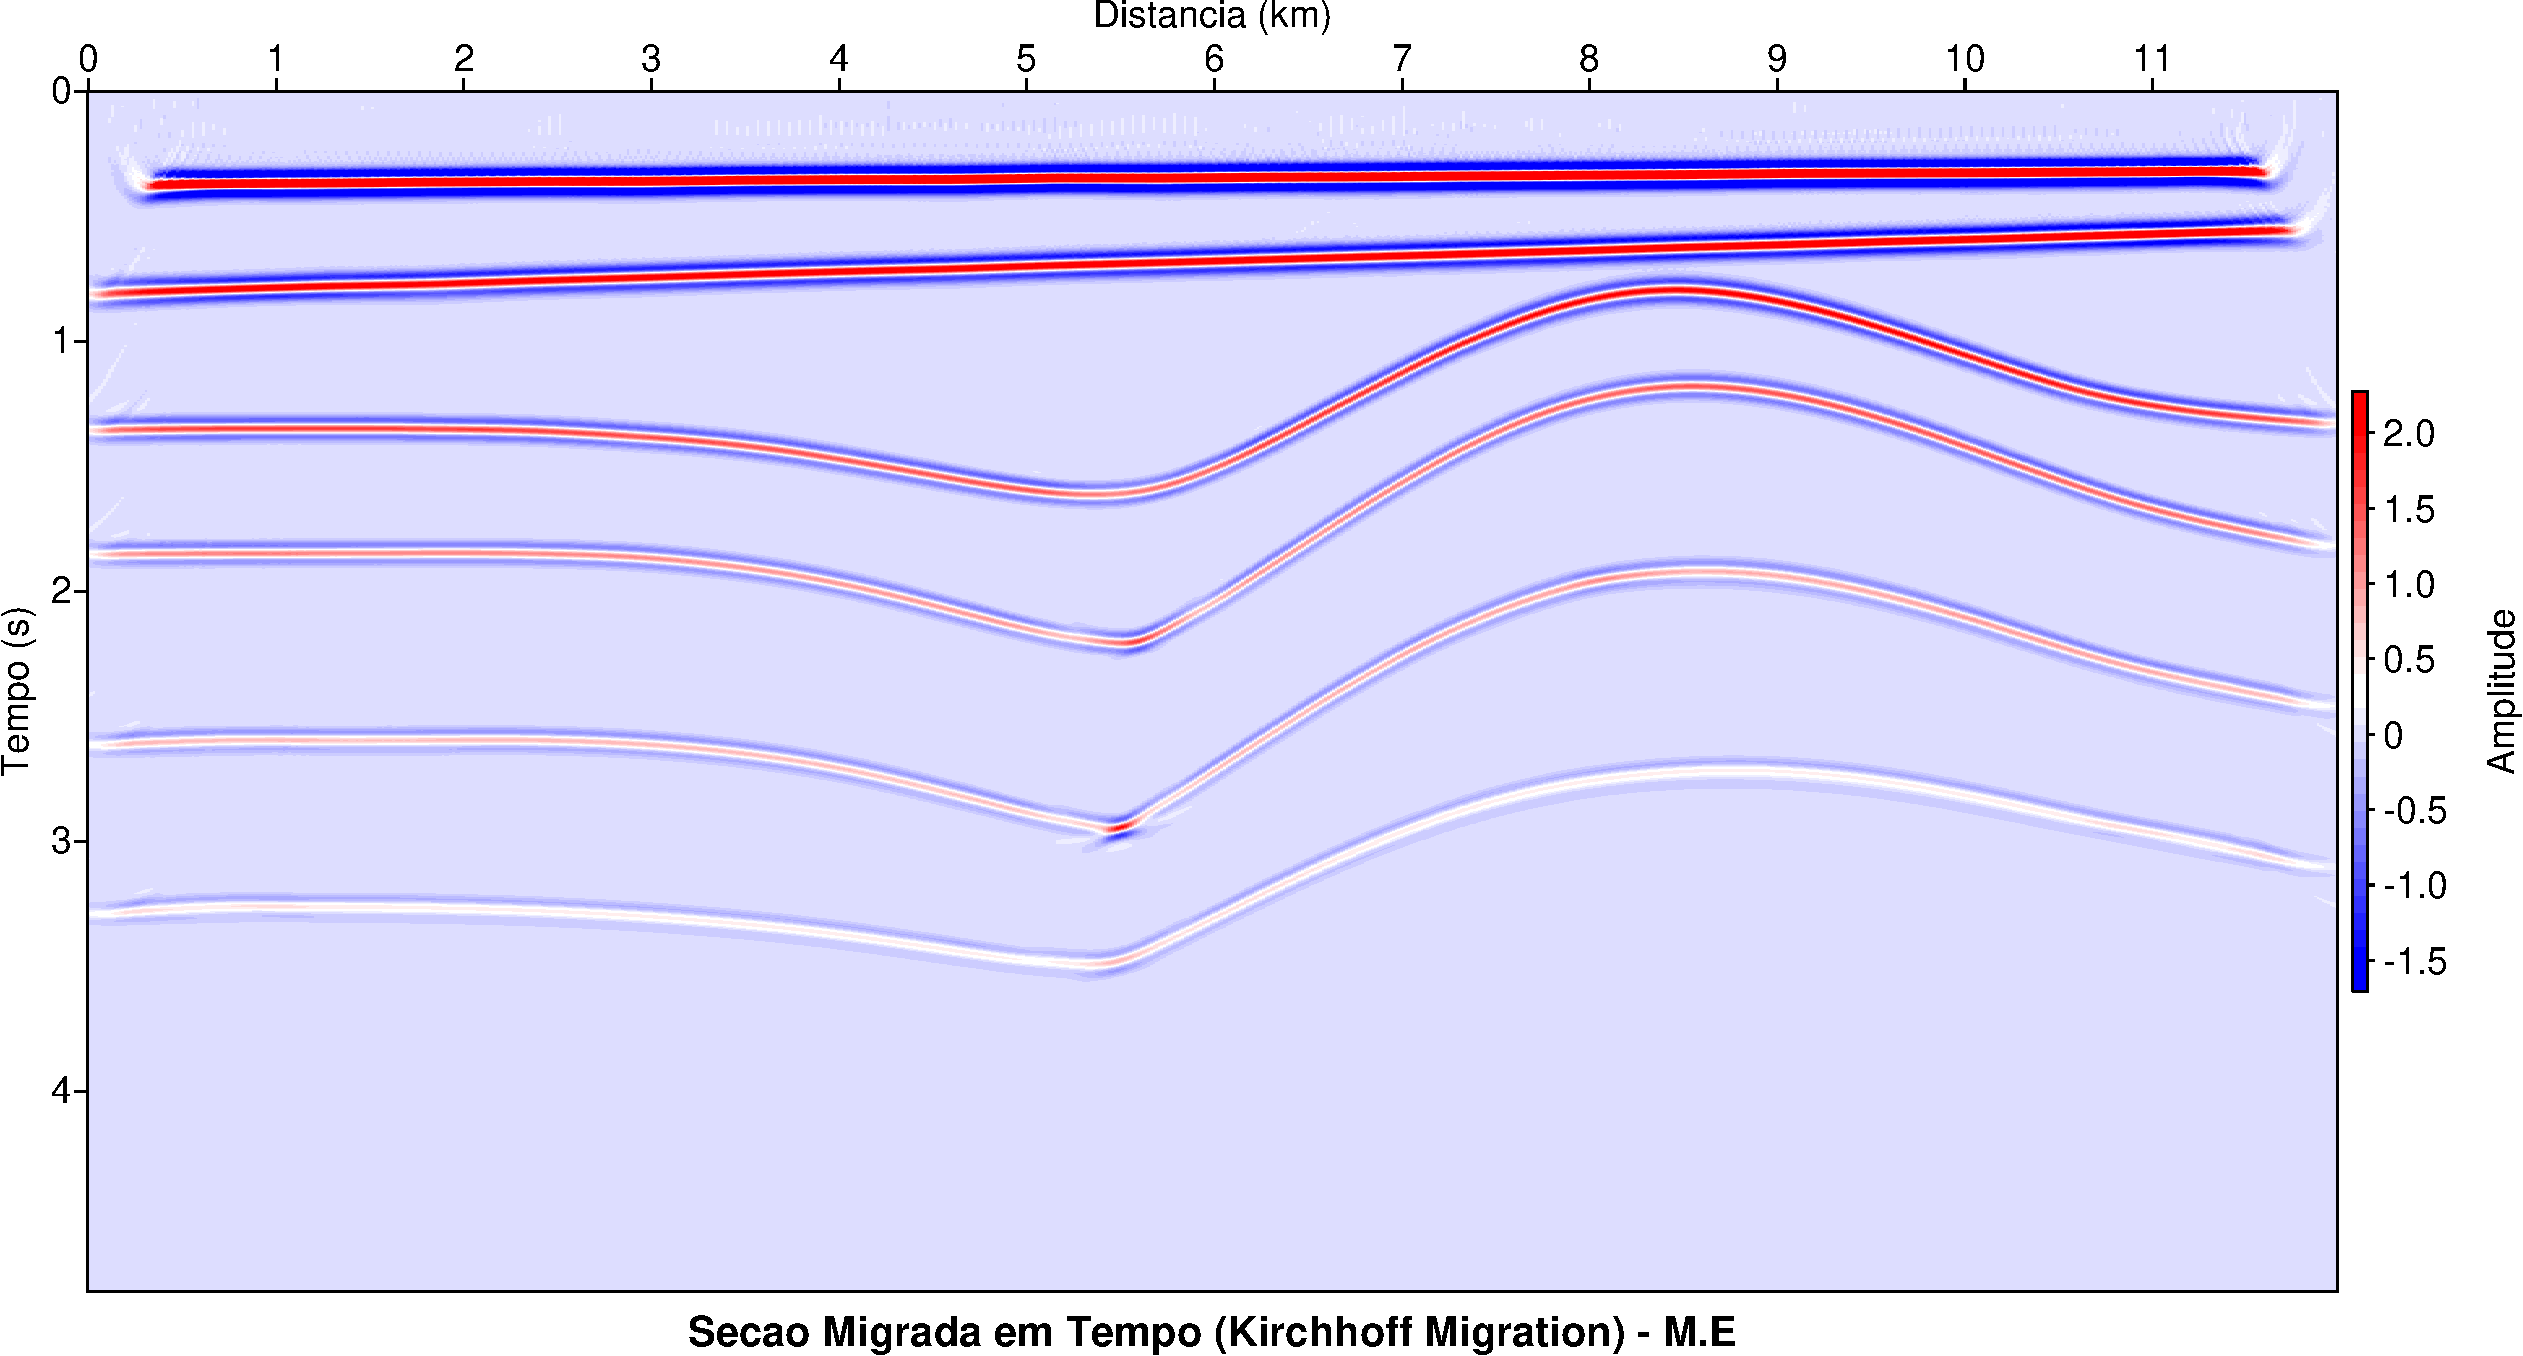
\includegraphics[totalheight=14cm]{figuras/cap3/seis_mig_time_ME.pdf}
\caption{Seção migrada em tempo pelo método Kirchhoff utilizando o modelo exato de velocidade (figura \ref{fig:modelo_velocidade}).}
\label{fig:seis_mig_time_ME}
\end{figure}
\end{landscape}

\section{MIGRAÇÃO DIFERENÇAS FINITAS EM PROFUNDIDADE}

Migração é o processo que cria uma imagem da subsuperfície a partir de dados sísmicos registrados em superfície, idealmente reposicionando os dados registrados em sua verdadeira posição geológica em subsuperfície. Existem duas abordagens principais para executar a migração: migração em tempo e migração em profundidade, que podem ser feitas após o processo de empilhamento ou antes do empilhamento.

A migração por diferenças finitas foi desenvolvida e popularizada por J. F. Claerbout, da Universidade de Stanford, e agora é amplamente utilizada no processamento sísmico. Para a maioria das seções, a migração de diferenças finitas fornece resultados comparáveis aos obtidos pela migração convencional de Kirchhoff e, onde os eventos não estão diminuindo muito, uma aparência mais limpa geralmente é aparente. No entanto, existem duas limitações práticas para o método, e elas ocorrem em regiões de mergulho muito acentuado e onde há uma grande variação da velocidade na direção lateral. \citep{HOOD(1978)}

O ponto de partida para a migração das ondas é normalmente a equação da onda escalar. Em um sistema de coordenadas em que o tiro e o receptor são coincidentes (ou seja, aproximadamente em uma pilha CDP), a velocidade deve ser reduzida pela metade \citep{Loewenthal(1976)}, de modo que nessas coordenadas a equação da onda seja:
\begin{equation}
\frac{\partial^{2} P}{\partial x^{2}}+\frac{\partial^{2} P}{\partial z^{2}}=\frac{4}{c^{2}} \frac{\partial^{2} P}{\partial t^{2}}
\label{eq:escalar_onda}
\end{equation}

onde $P(x, z, t)$ é a pressão registrada nos hidrofones, $x$, $z$, $t$ são as coordenadas horizontal, vertical e de tempo, respectivamente, e $c(x, z)$ é a velocidade de ondas.

A equação de onda unidirecional que governa a propagação de ondas ao longo da direção do eixo $z$ é (no domínio da frequência):
\begin{equation}
\frac{\partial P}{\partial z}=i\left(\frac{4\omega^{2}}{c^{2}}+\frac{\partial^{2}}{\partial x^{2}}\right)^{1/2} P=iSP
\label{eq:freq_onda}
\end{equation}

onde $\omega$ é a frequência angular.

A chave para o sucesso de várias aproximações parabólicas da equação (\ref{eq:freq_onda}) reside na precisão com a qual o termo raiz quadrada $S$ is é aproximado. Claerbout (1970) deriva um conjunto de aproximações de várias ordens, e na figura \ref{fig:df2} as aproximações de segunda e terceira ordem para a raiz quadrada são mostradas. Estes são chamados as aproximações de $15^{\circ}$ e $45^{\circ}$, respectivamente.

\begin{figure}[H]
\centering
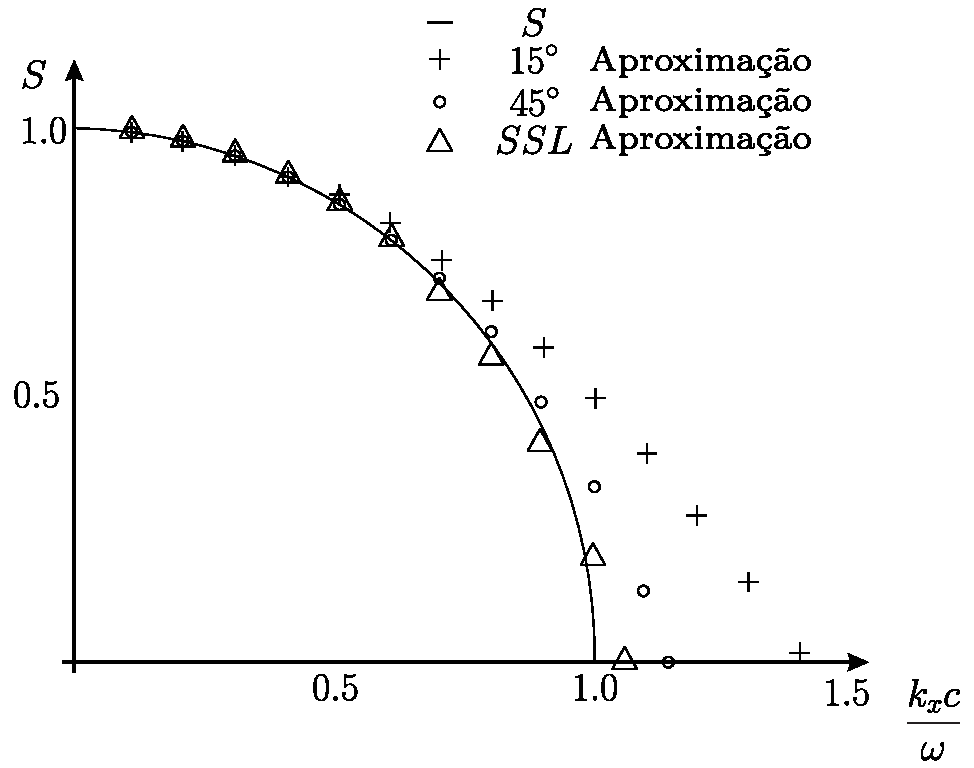
\includegraphics[height=8.0cm]{figuras/cap3/df2.pdf}
\caption{Aproximações para o termo $S$ da equação (\ref{eq:freq_onda}). Figura modificada de \citep{HOOD(1978)}.}
\label{fig:df2}
\end{figure}

É possível usar aproximações de quarta ordem ou superiores a $S$, mas há várias desvantagens computacionais decorrentes do fato de que as equações de diferenças finitas resultantes não têm mais uma forma tridiagonal direta. Isso causa um aumento progressivo nos custos computacionais. Além disso, os erros introduzidos pelo método das diferenças finitas podem ser mais graves do que os causados pela equação da onda parabólica, de modo que, a menos que o método das diferenças finitas seja abandonado em favor de outras técnicas, parece haver poucas perspectivas de aproximações de alta ordem que atinjam qualquer melhoria notável \citep{HOOD(1978)}.


Voltando agora à equação (\ref{eq:freq_onda}), uma equação de $15^{\circ}$ é derivada para referência posterior. Seja $c$ uma velocidade constante. Nós temos então
\begin{align}\nonumber
\frac{\partial P}{\partial z}&=\mathrm{i} \frac{2 \omega}{c}\left[\mathrm{I}-\mathrm{I}+\left(\frac{\bar{c}}{c}\right)^{2}+\left(\frac{\bar{c}}{2 \omega}\right)^{2} \frac{\partial^{2}}{\partial x^{2}}\right]^{1 / 2} P\\
\label{eq:velocidade_const}&=\mathrm{i}\frac{\omega}{\bar{c}}\left[\mathrm{I}+\left(\frac{\bar{c}}{c}\right)^{2}+\left(\frac{\bar{c}}{2 \omega}\right)^{2} \frac{\partial^{2}}{\partial x^{2}}\right] P
\end{align}

Esta pode ser colocada em um período de tempo retardado, configurando $P=P^{\prime} \exp (\mathrm{i} 2 \omega z / \bar{c})$ portanto:
\begin{align}
\frac{\partial P^{\prime}}{\partial z}=\mathrm{i} \frac{\omega}{\bar{c}}\left[\left(\frac{\bar{c}}{c}\right)^{2}-\mathrm{I}+\left(\frac{\bar{c}}{2 \omega}\right)^{2} \frac{\partial^{2}}{\partial x^{2}}\right] P^{\prime}
\label{eq:tempo_retard}
\end{align}

Restaurando (\ref{eq:tempo_retard}) o domínio do tempo e eliminando os primos, obtemos:
\begin{align}
\frac{\partial^{2} P}{\partial t \partial z}=\frac{\partial^{2} P}{\partial t^{2}}\left(\frac{\bar{c}}{c^{2}}-\frac{1}{\bar{c}}\right)-\frac{\bar{c}}{4} \frac{\partial^{2} P}{\partial z^{2}}
\label{eq:sem_primo}
\end{align}

Um caso especial disso ocorre se as variações de velocidade lateral são insignificantes; nesse caso, negligenciando os efeitos de transmissão, a seguinte equação pode ser derivada:
\begin{align}
\frac{\partial^{2} P}{\partial z \partial t}=-\frac{c(z)}{4} \frac{\partial^{2} P}{\partial x^{2}}
\label{eq:desprez_termos}
\end{align}

Seja $P_{j, k, n}$ o valor de $P$ no ponto de malha $P(t_j, x_k, z_n)$. Os seguintes operadores de diferença podem ser definidos:
\begin{align*}
D_{x} P_{j, k, n}&=\left(P_{j, k+1, n}-P_{j, k, n}\right) \frac{\mathrm{I}}{\Delta x} \quad \left(\approx \frac{\partial P}{\partial x}\right),\\
D_{x x} P_{j, k, n}&=\left(P_{j, k+1, n}-2 P_{j, k, n}+P_{j, k-1, n}\right) \frac{\mathrm{I}}{\Delta x^{2}} \quad \left(\approx \frac{\partial^{2} P}{\partial x^{2}}\right),
\end{align*}


organizando desta forma 
\begin{align*}
A_{1} P_{j, k, n} &=\frac{1}{2}\left[(\mathrm{I}-\theta) P_{j, k, n}+\theta P_{j, k, n+1}\right.\\ &\left.+(\mathrm{I}-\theta) P_{j+1, k, n}+\theta P_{j+1, k, n+1}\right],
\end{align*}

e
\begin{align*}
A_{2} P_{j, k, n}=\alpha P_{j, k+1, n}+(\mathrm{I}-2 \alpha) P_{j, k, n}+\alpha P_{j, k-1, n}
\end{align*}


A equação (\ref{eq:desprez_termos}) pode ser expressa em notação de diferencial como:
\begin{align}
\left(A_{2} D_{z} D_{t}+\frac{c(z)}{4} D_{x x} A_{1}\right) P_{j, k, n}=0
\label{eq:diferencial_fd}
\end{align}

Para estabilidade da equação (\ref{eq:diferencial_fd}) $0 \leqslant \alpha \leqslant \frac{1}{4}$ e $0.5 \leqslant \theta \leqslant \mathrm{I}$ É necessário. Valores de $\alpha$ na faixa $\frac{1}{12} \leqslant \alpha \leqslant \frac{1}{6}$ parece ser amplamente aceito \citep{Claerbout(1985)}.

Para inclusão dos efeitos da variação da velocidade lateral o método utilizado envolve uma conversão da seção em ``tempo'' para uma seção ``profundidade''. Assim, em vez de usar o sistema de coordenadas deslocadas no tempo usual:
\begin{align*}
t^{\prime}=t+\frac{z}{c}
\end{align*}

uma coordenada de profundidade $d$ é usada definida por:
\begin{align*}
d=\frac{c_{a} t}{2}+z
,
\end{align*}

onde $c_{a} t=\int_{0}^{t} c_{int} \mathrm{d} t$

$c_{a}$ é comumente referido como a velocidade média e $c_{int}$ como a velocidade do intervalo. Desde que a velocidade do intervalo varie lentamente em função da $x$ e $z$.


\begin{landscape}
\begin{figure}[H]
\centering
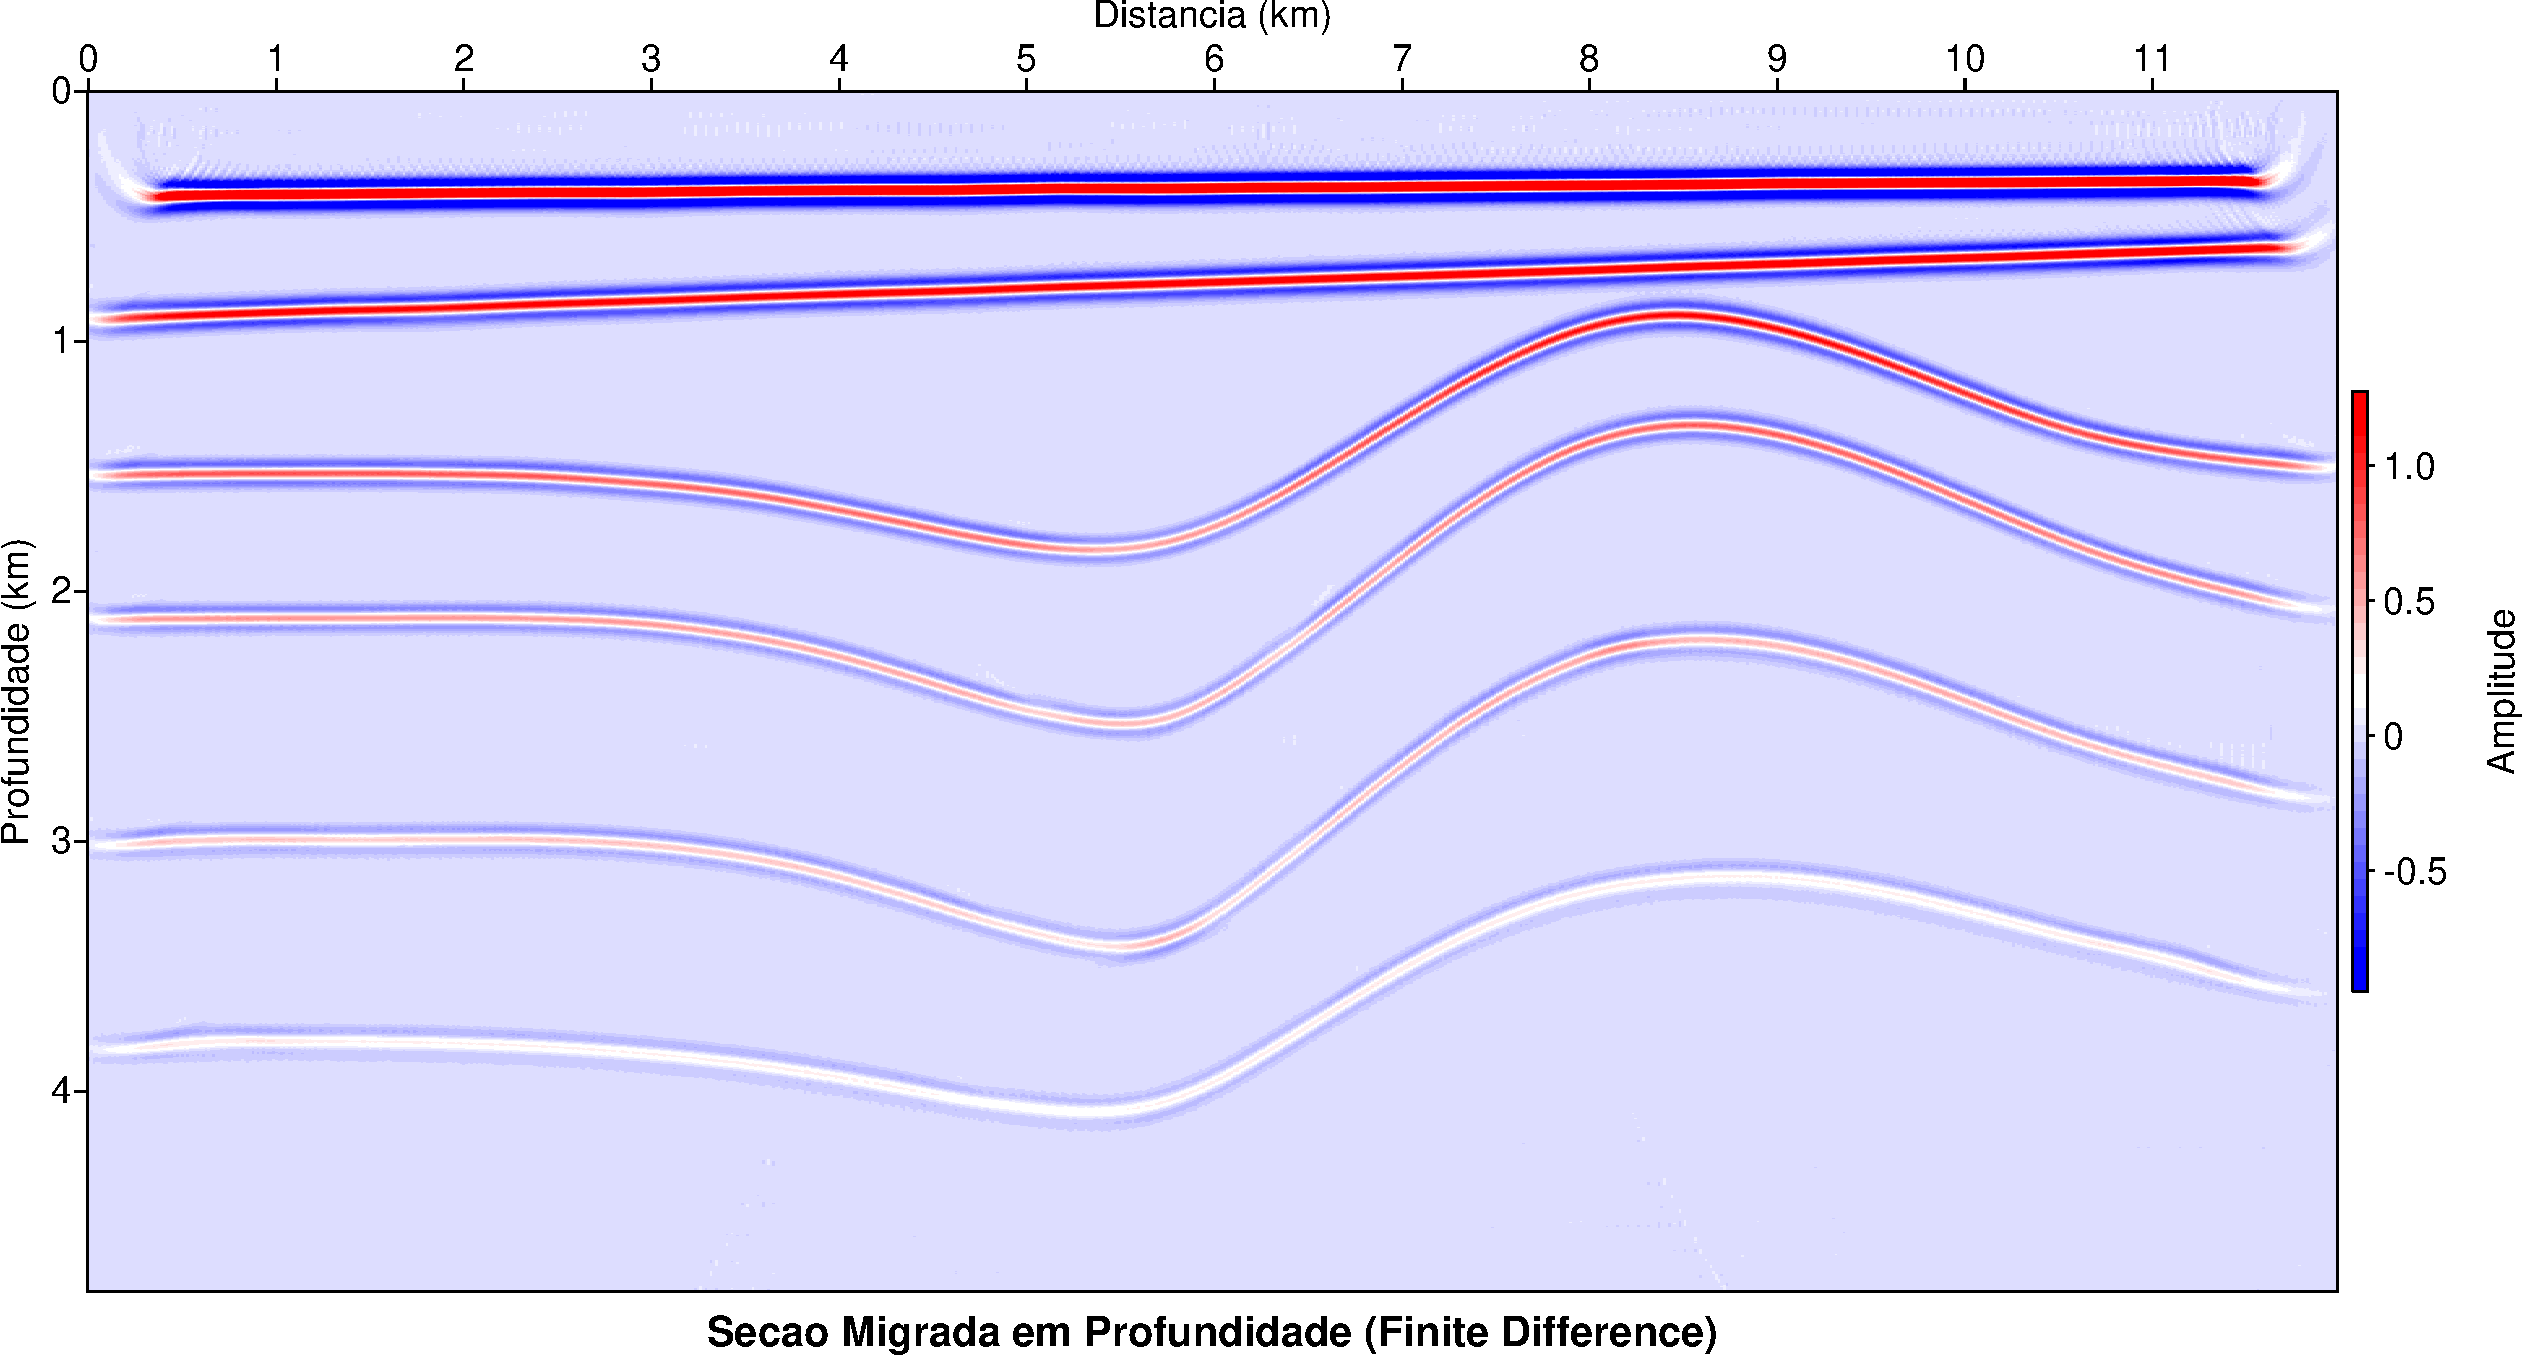
\includegraphics[totalheight=14cm]{figuras/cap3/seis_mig_deph_fd.pdf}
\caption{Seção migrada em tempo pelo método Diferenças Finitas utilizando o modelo de velocidade suavizado.}
\label{fig:seis_mig_deph_fd}
\end{figure}
\end{landscape}

\begin{landscape}
\begin{figure}[H]
\centering
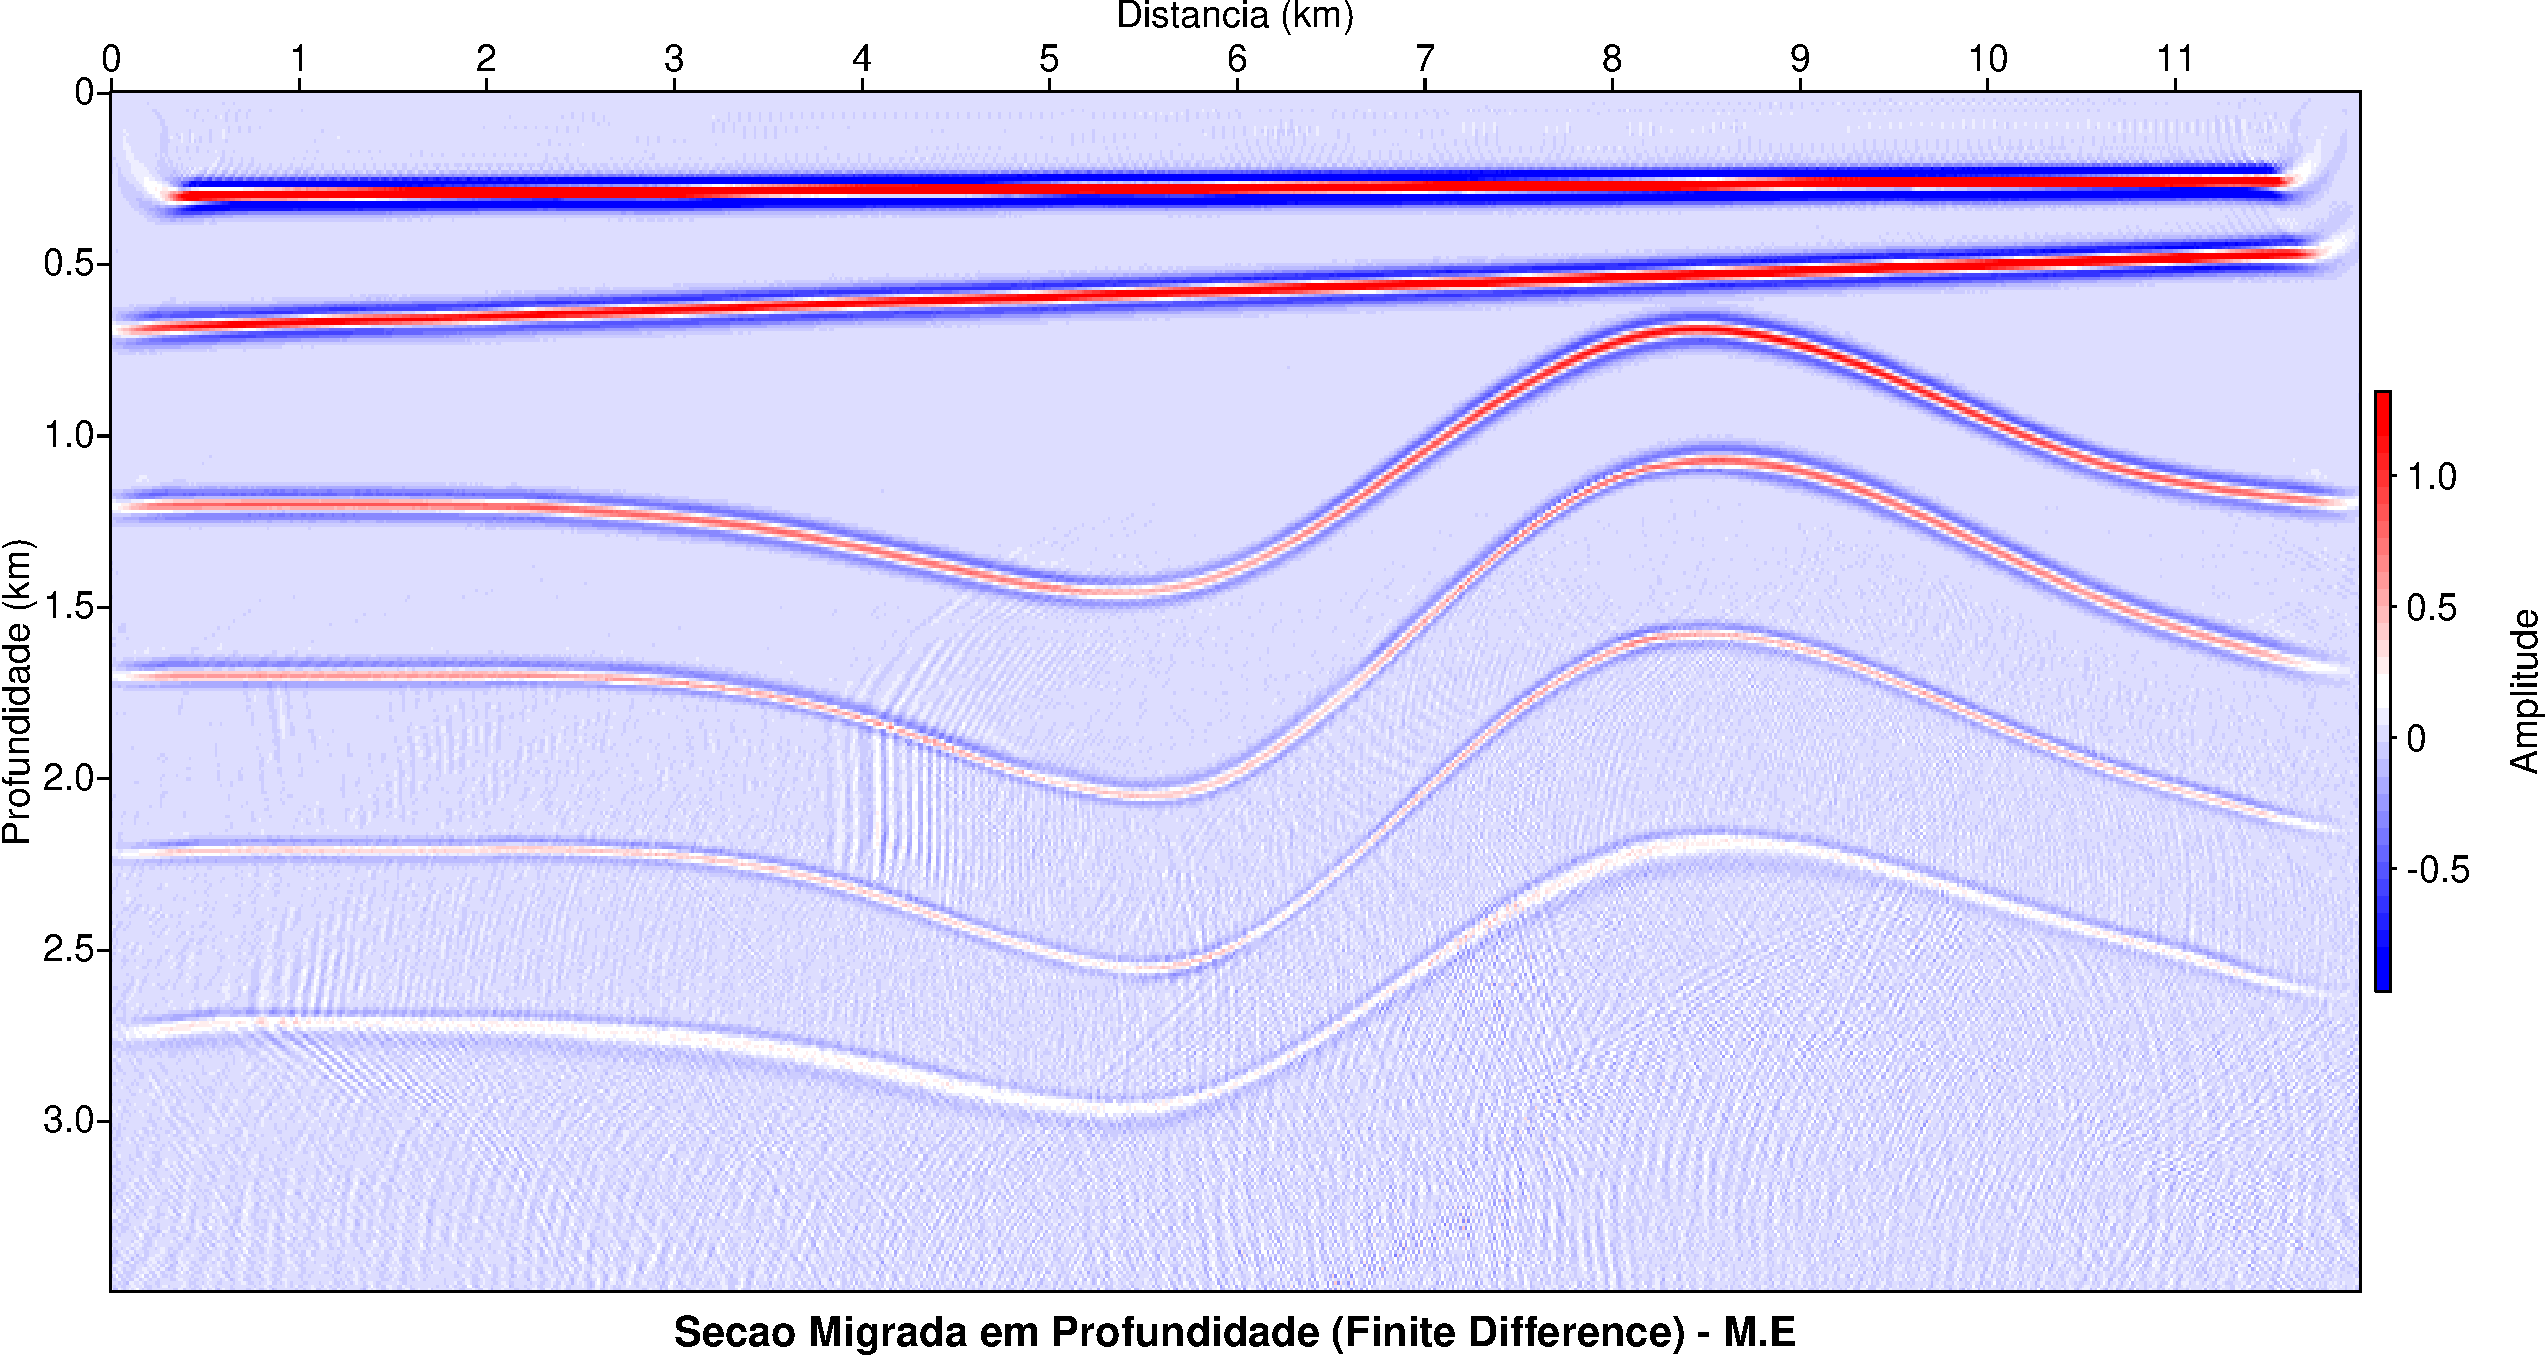
\includegraphics[totalheight=14cm]{figuras/cap3/seis_mig_depth_fd_me.pdf}
\caption{Seção migrada em tempo pelo método Diferenças Finitas utilizando o modelo exato de velocidade (figura \ref{fig:modelo_velocidade}).}
\label{fig:seis_mig_depth_fd_me}
\end{figure}
\end{landscape}

\section{OUTRAS METODOLOGIAS DE MIGRAÇÃO EM PROFUNDIDADE}

Nesta seção propõe-se utilizar outras metodologias de migração em profundidade para comparação com o dado migrado por diferenças finitas.

A equação de onda escalar unidirecional é a base para algoritmos de migração comuns. Esses algoritmos não modelam explicitamente várias reflexões, ondas convertidas, ondas de superfície ou ruído. Qualquer energia presente na entrada de dados para migração é tratada como reflexões primárias. Os algoritmos de migração podem ser classificados em três categorias principais: \citep{Yilmaz(2000)}

\begin{enumerate}
 \item Aqueles que se baseiam na solução integral para o equação de onda escalar,
 \item Aqueles que são baseados nas soluções de diferenças finitas, e
 \item Aqueles baseados em implementações de número de onda de frequência.
\end{enumerate}

Qualquer que seja o algoritmo, deve:
\begin{enumerate}
 \item Lidar com quedas acentuadas com precisão suficiente,
 \item Lidar com variações de velocidade lateral e vertical, e
 \item Ser implementado com eficiência.
\end{enumerate}

\begin{landscape}
\begin{figure}[H]
\centering
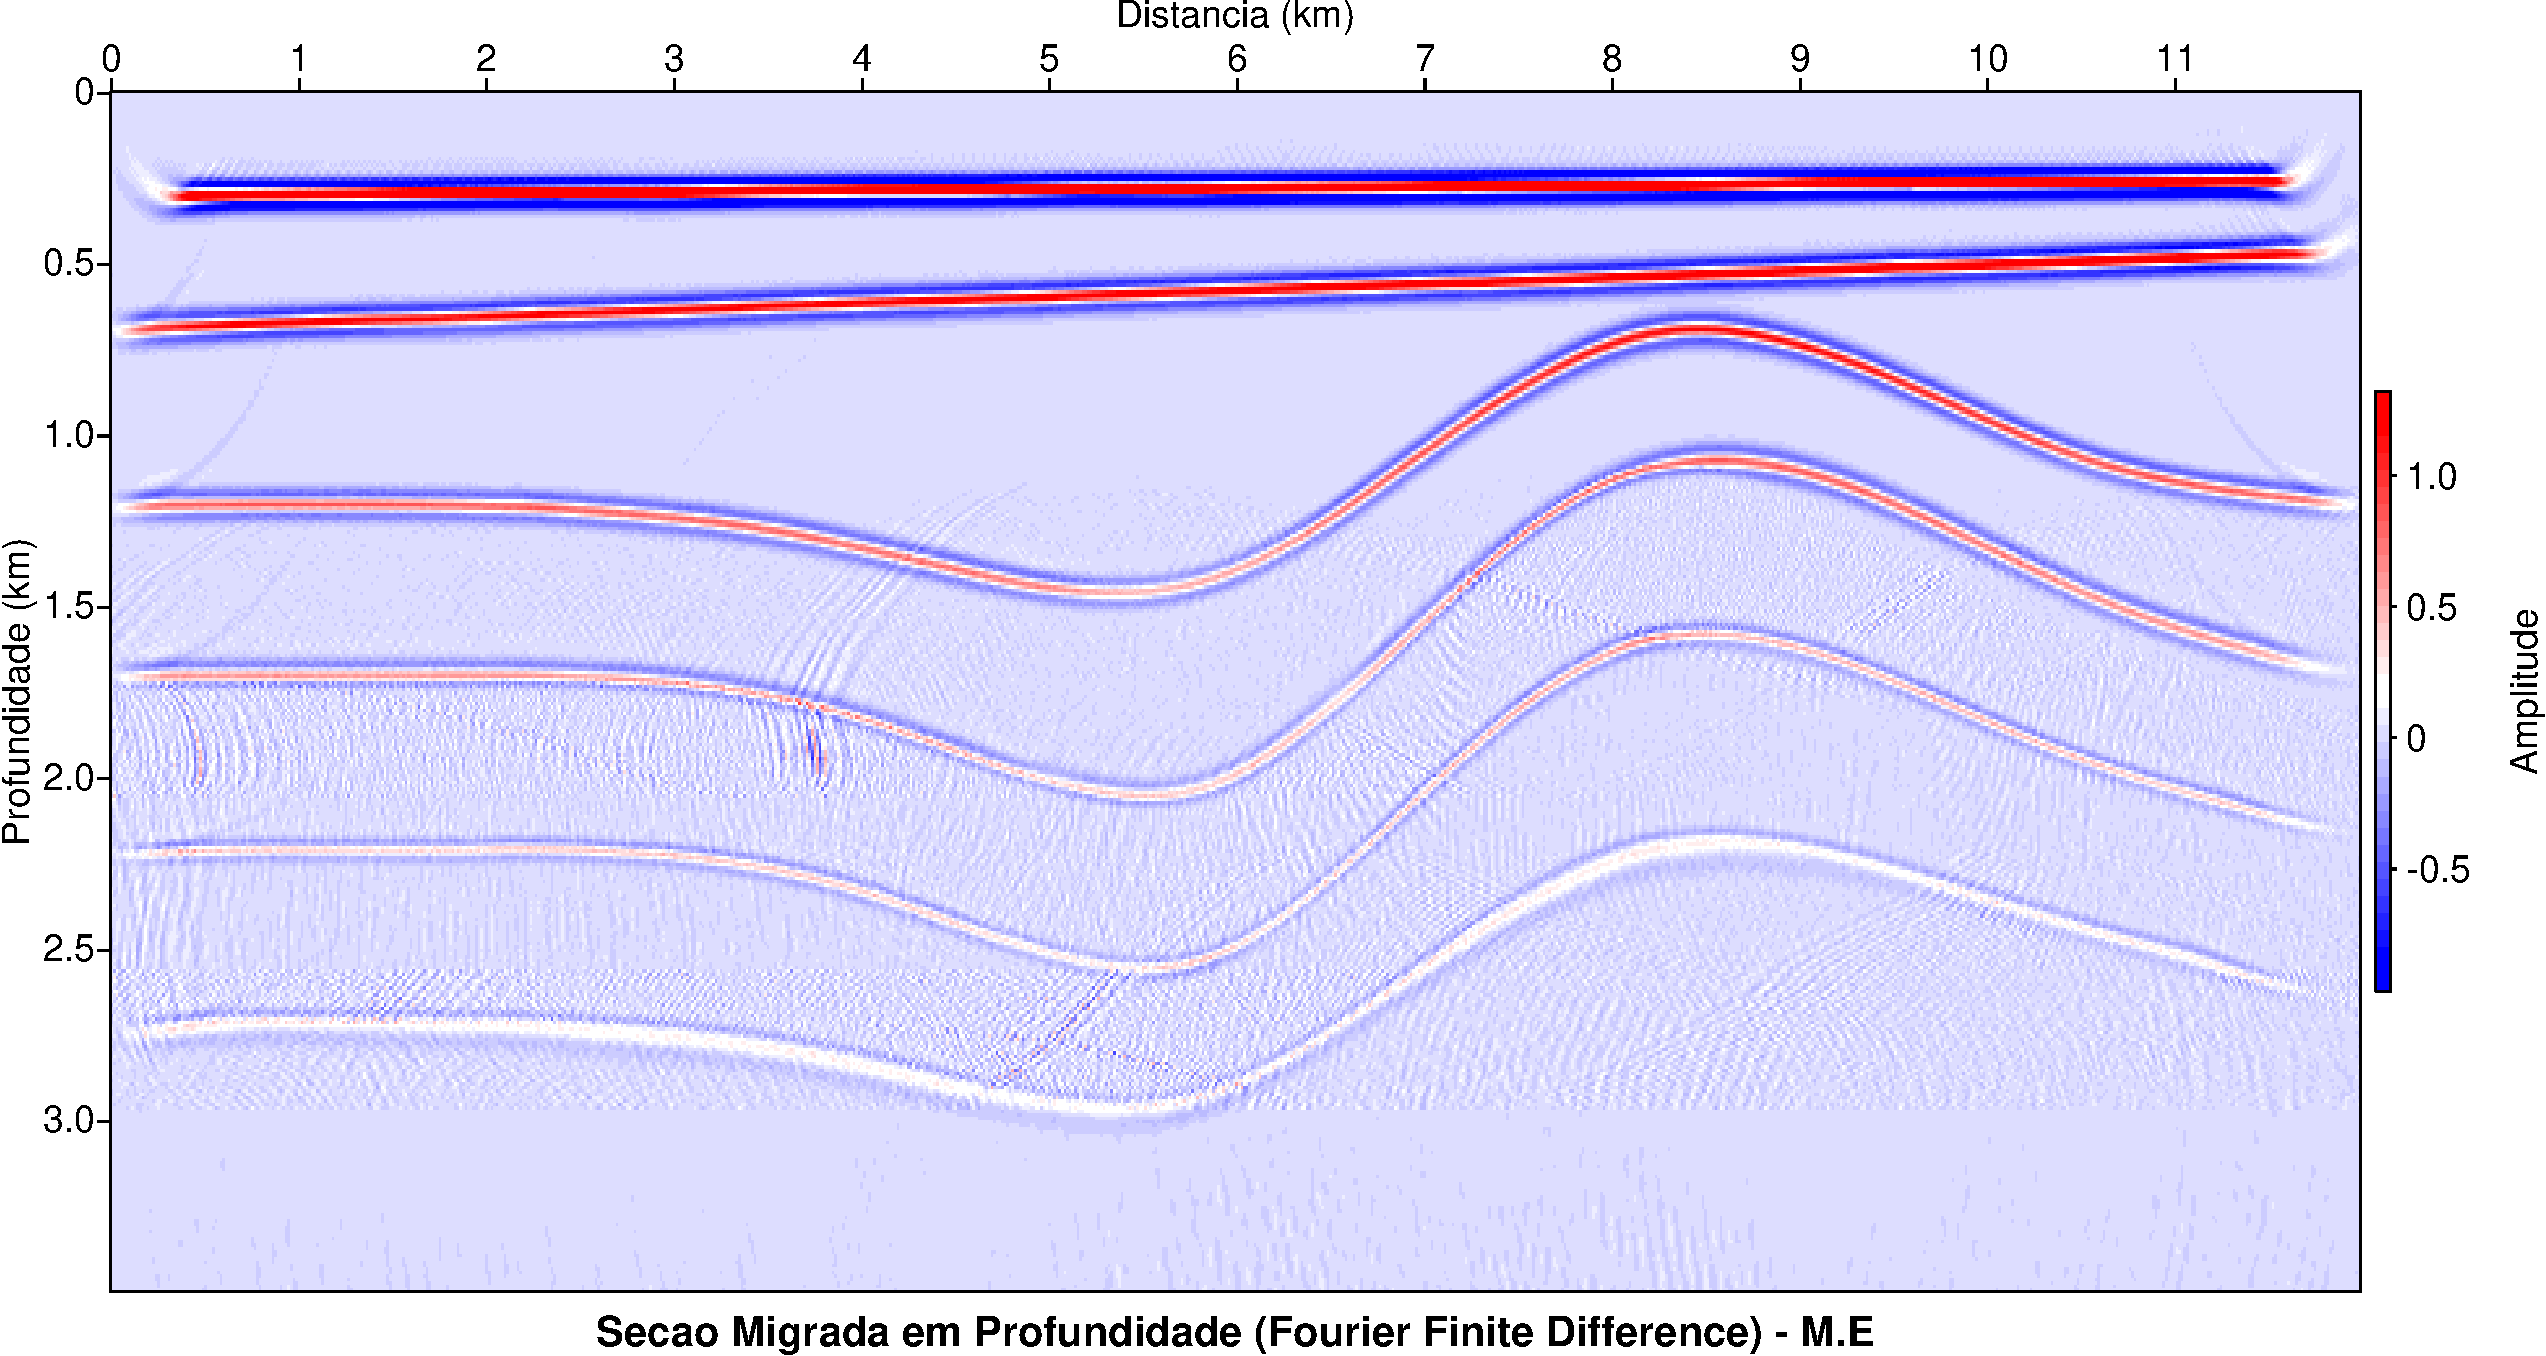
\includegraphics[totalheight=14cm]{figuras/cap3/seis_Mig_FFD_depth_me.pdf}
\caption{Seção migrada em tempo pelo método FFD utilizando o modelo exato de velocidade (figura \ref{fig:modelo_velocidade}).}
\label{fig:seis_mig_depth_fd_me}
\end{figure}
\end{landscape}

\begin{landscape}
\begin{figure}[H]
\centering
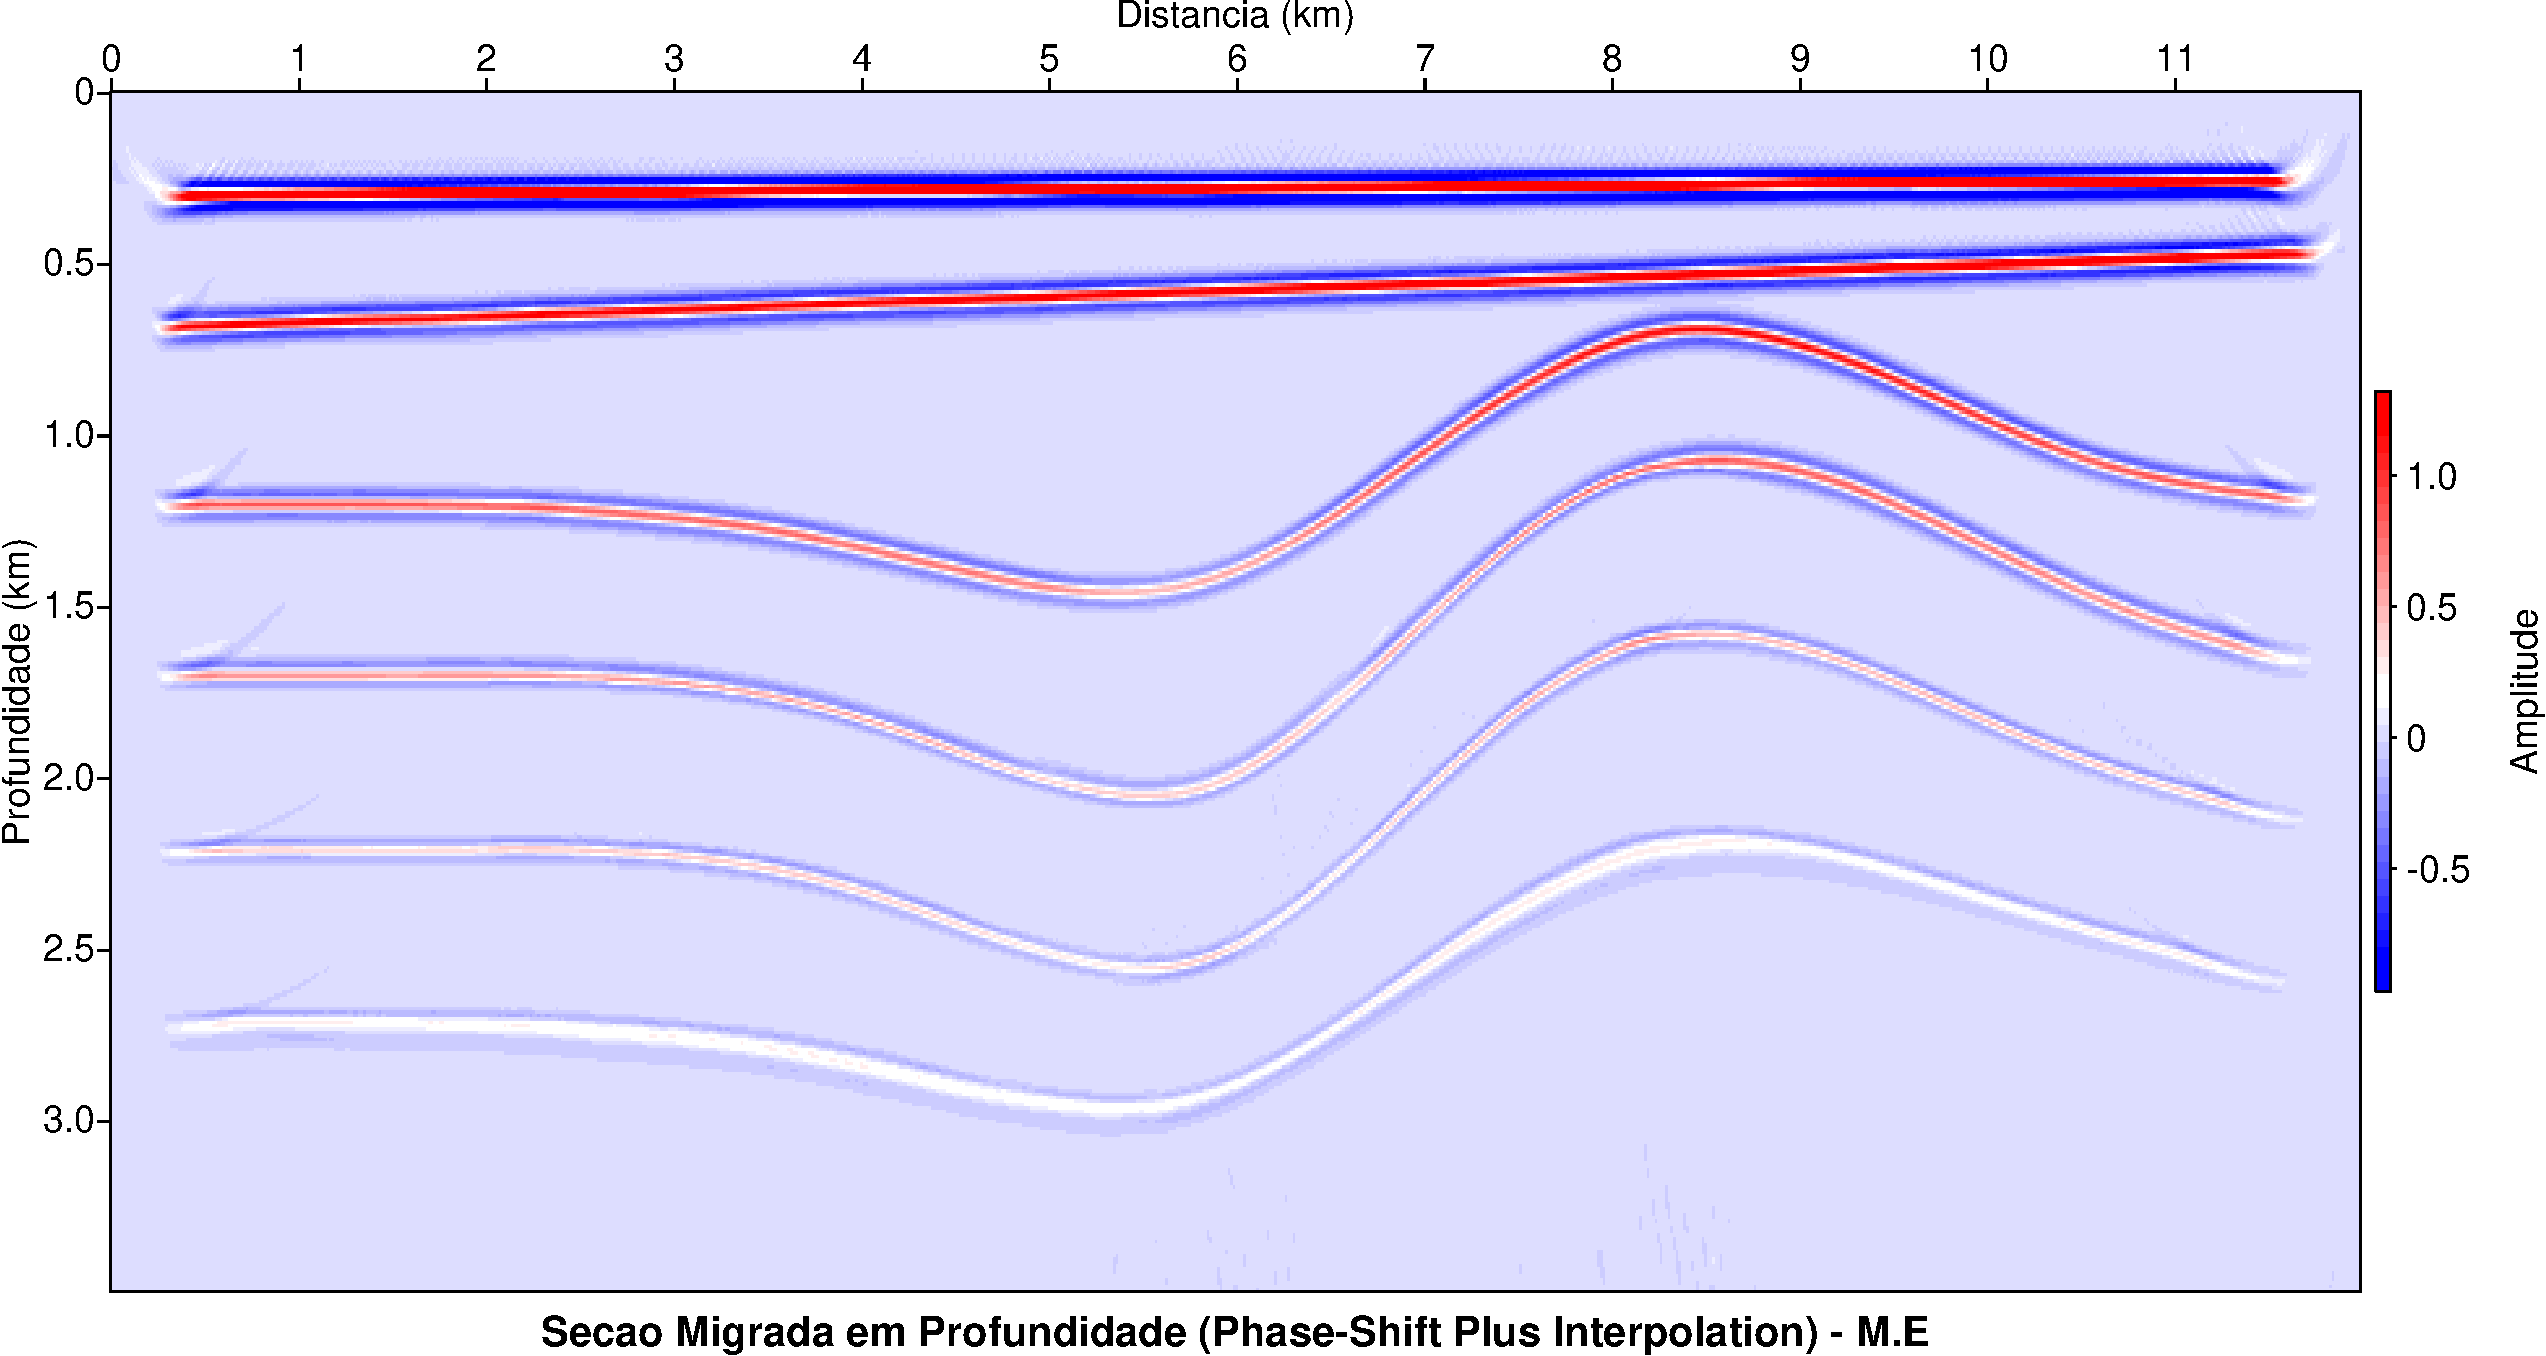
\includegraphics[totalheight=14cm]{figuras/cap3/seis_Mig_PSPI_depth_me.pdf}
\caption{Seção migrada em tempo pelo método PSPI utilizando o modelo exato de velocidade (figura \ref{fig:modelo_velocidade}).}
\label{fig:seis_mig_depth_fd_me}
\end{figure}
\end{landscape}

\begin{landscape}
\begin{figure}[H]
\centering
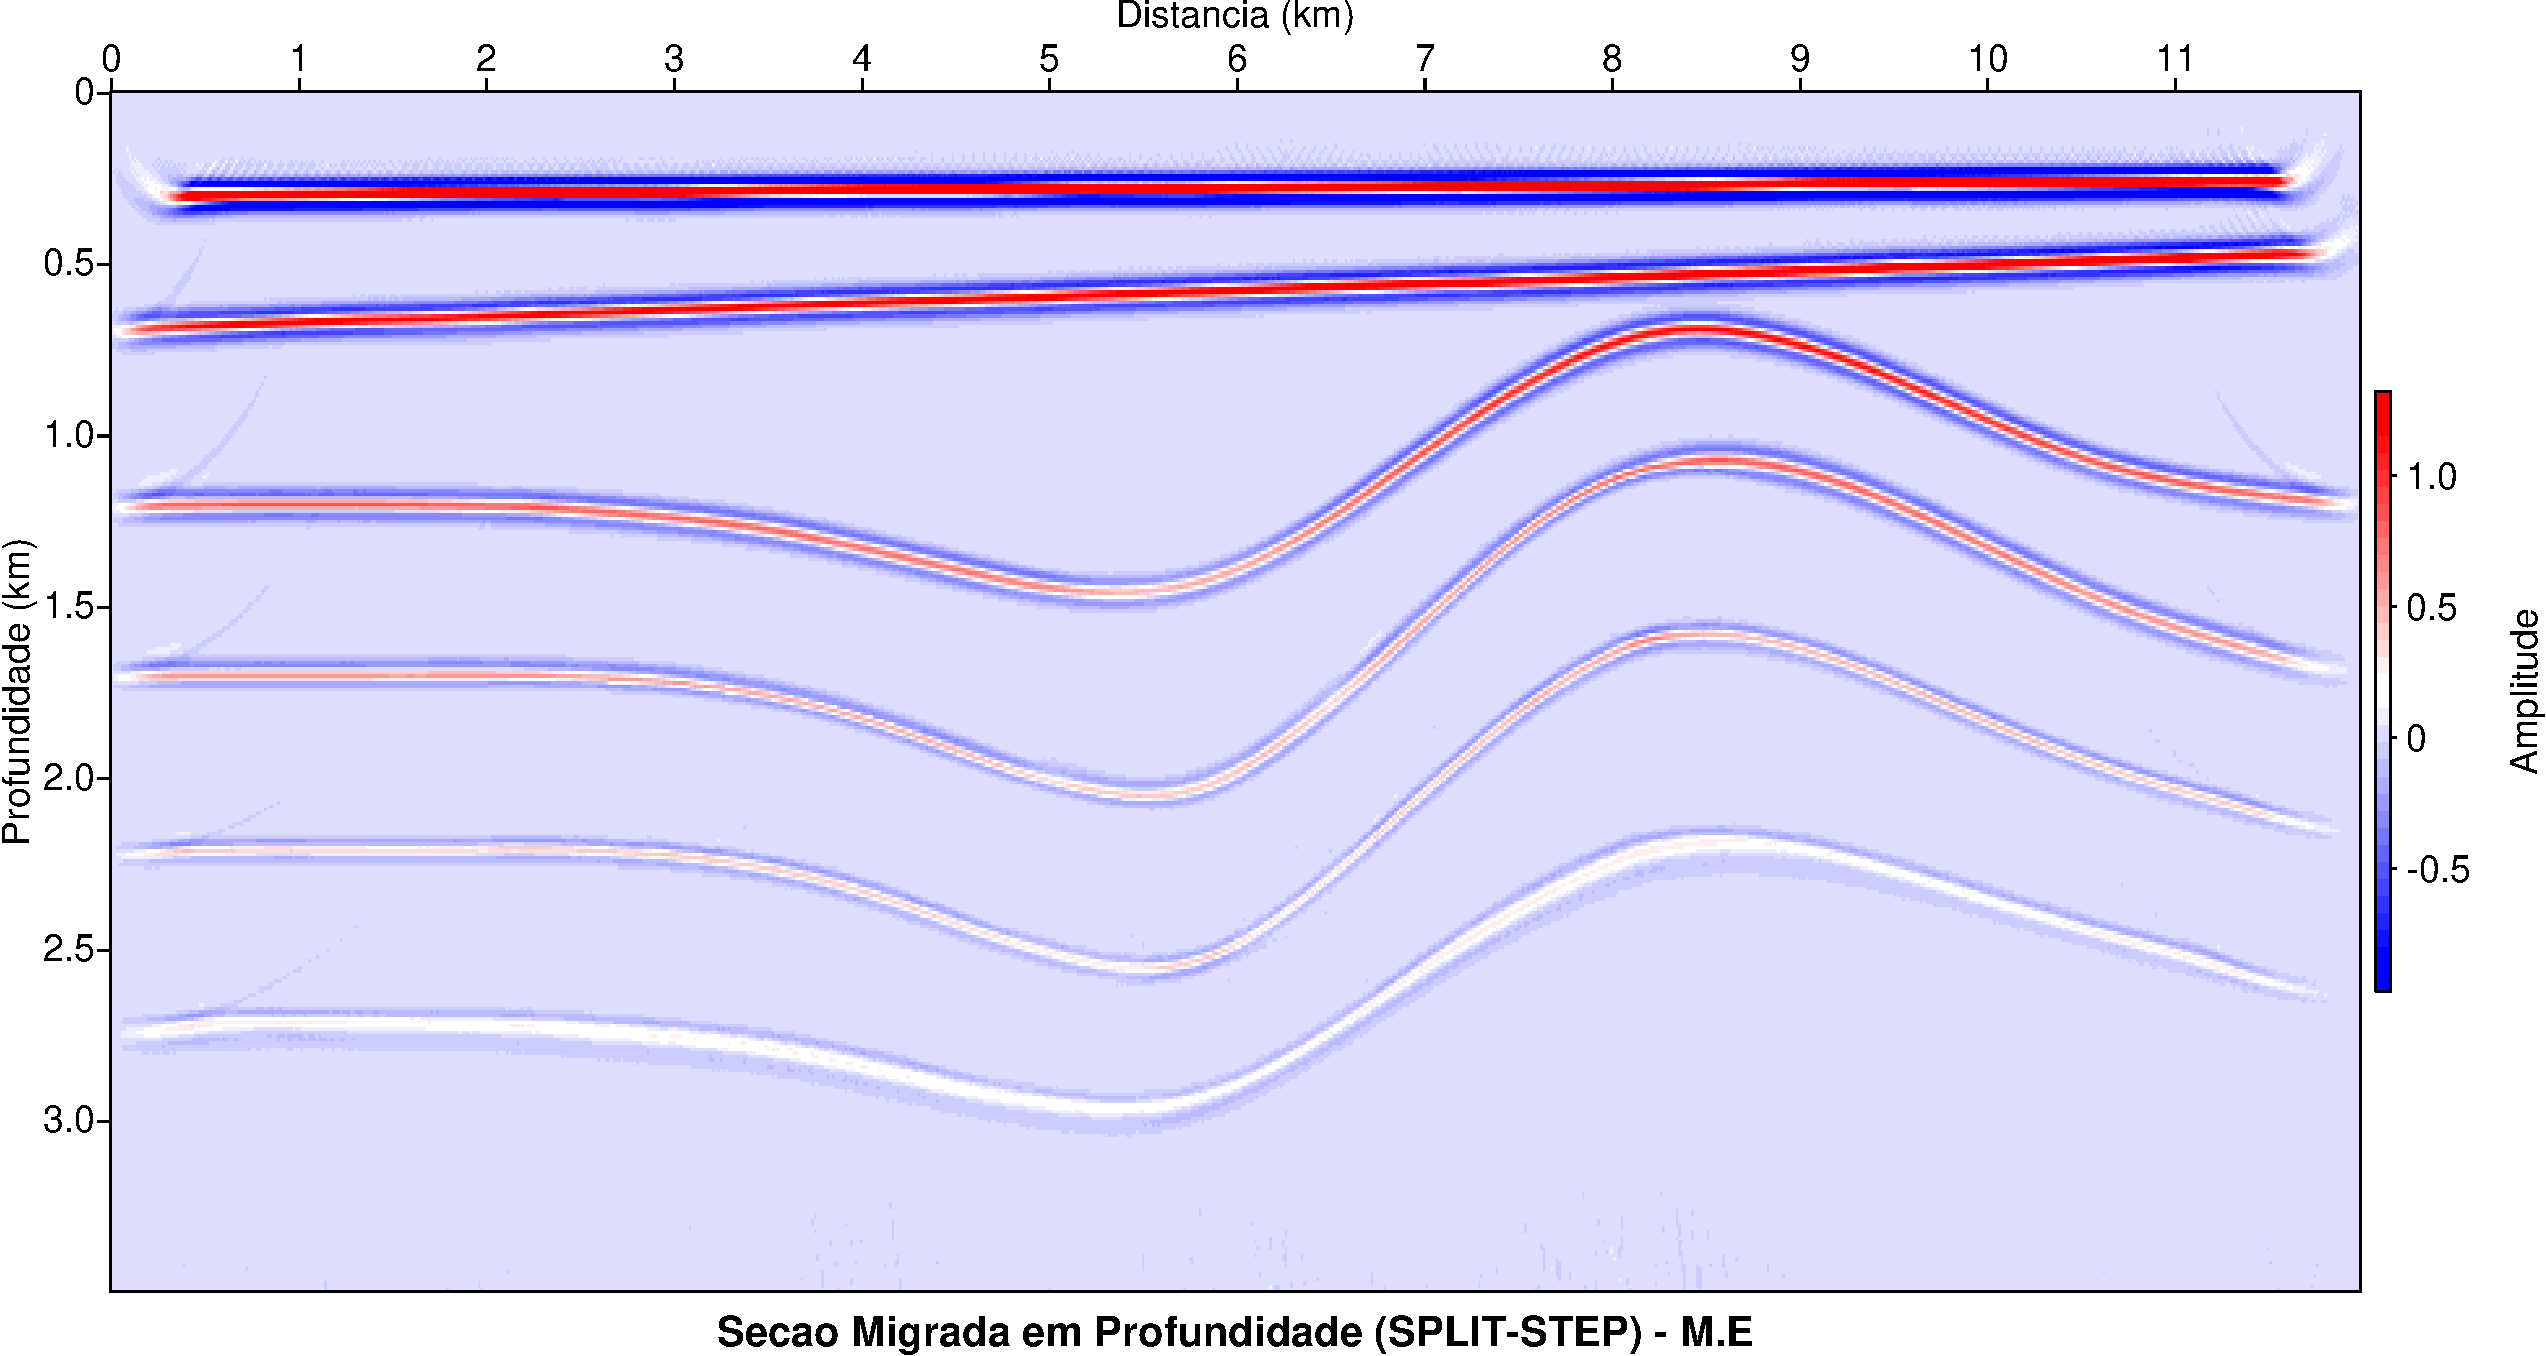
\includegraphics[totalheight=14cm]{figuras/cap3/seis_Mig_SPLIT_STEP_depth_me.pdf}
\caption{Seção migrada em tempo pelo método SPLIT STEP utilizando o modelo exato de velocidade (figura \ref{fig:modelo_velocidade}).}
\label{fig:seis_mig_depth_fd_me}
\end{figure}
\end{landscape}
